\documentclass[ms,english]{stthesis}
\usepackage{lipsum}
\usepackage[color=green]{todonotes}
\usepackage{graphicx}
\usepackage{subcaption}
\usepackage{multirow}
\usepackage{booktabs}
\usepackage{epigraph}
\usepackage{cite}
\usepackage[acronym]{glossaries}
\usepackage[most]{tcolorbox}
\usepackage{hyperref}

% \usepackage[table]{xcolor}
\usepackage{float}

\usepackage{amssymb}
% \usepackage{wasysym}

\usepackage{xspace}
\usepackage{pifont}% http://ctan.org/pkg/pifont
\newcommand{\cmark}{\ding{51}}%
\newcommand{\xmark}{\ding{55}}%

\makeglossaries
% --- MOEA
\newglossaryentry{moea}{type=\acronymtype, name={MOEA}, description={Multi-objective evolutionary algorithm}, first={Multi-objective evolutionary algorithm (MOEA)}}

% --- MOO
\newglossaryentry{moo}{type=\acronymtype, name={MOO}, description={multi-objective optimization}, first={multi-objective optimization (MOO)}}

% --- EA
\newglossaryentry{ea}{type=\acronymtype, name={EA}, description={Evolutionary algorithm}, first={Evolutionary algorithm (EA)}}







\newglossaryentry{apig}{name={API},
    description={An Application Programming Interface (API) is a particular set
of rules and specifications that a software program can follow to access and
make use of the services and resources provided by another particular software
program that implements that API}}

%%% define the acronym and use the see= option
\newglossaryentry{api}{type=\acronymtype, name={API}, description={Application
Programming Interface}, first={Application
Programming Interface (API)\glsadd{apig}}, see=[Glossary:]{apig}}


% "No Free Lunch" (NFL) theorems demonstrate that if an algorithm performs well on a certain class of problems then it necessarily pays for that with degraded performance on the set of all remaining problems Additionally, the name emphasizes the parallel with similar results in supervised learning.

\newcommand{\todor}[1]{\todo[color=green,inline,size=\small]{Reviewer: #1}}
\newcommand{\todoy}[1]{\todo[color=yellow,size=\small]{Oleksandr: #1}}

\definecolor{block-gray}{gray}{0.85}
\newtcolorbox{blockquote}{colback=block-gray,grow to right by=-1mm,grow to left by=-1mm,boxrule=0pt,boxsep=0pt,breakable}

\title{Compositional multi-objective parameter tuning}
\author{Oleksandr Husak}
\date{\today}
\birthday{16.04.1994}
\birthplace{Ukraine}
\supervisor{MSc. Dmytro Pukhkaiev \newline Dr.-Ing. Sebastian Götz}


\begin{document}
    \maketitle % This sets the title page
  
    \tableofcontents
    % \listoffigures
    % \listoftables

    \section{Abstract}
Please stand by
    \chapter{Introduction}\label{sec:intro}

\begin{blockquote}
\paragraph{Intent:} A short version of thesis and a description of done work. Challenges and Problems.

    \begin{description}
        \item[1. Motivation] Surrogate model for multi-objective expensive black-box problem $\rightarrow$ Research gap: Portfolio/Compositional system/Sampling plan. Definition and motivation of the goal. Goal: MO solution $\rightarrow$ Problem: Expensive black-box $\rightarrow$ Solution: Answer research questions
        \item[2. Objectives of work] ?
        \item[3. Research Questions] Question from research gap. The answer to this questions is the purpose of the thesis
        \item[4. Results overview] A short overview of done work
    \end{description}
\end{blockquote}

% --------------------------------------------------------------------------------------------
% ------------------------------------------------     Motivation      
% --------------------------------------------------------------------------------------------
\section{Motivation}

    In traditional manual parameter tuning, engineers put the effort in searching the optimal objectives guided by experience and intuition. Regardless, many of these optimization problems have a huge search space that could be handled only with automatic tools. This kind of software could extrapolate and highlight the most perspective parameters from infinite space, but at the same time, struggle in multi-criteria decisions that are critical for engineering problems. For examples: architecture design, test generating, tuning machine-learning algorithms or experiment plan could be stated as multi-objective problems. To understand the space of possible solution, they are represented on the Pareto frontier; i.e. the subset os solutions that could be not improved in some objectives without degrading in another.
    Multi-objective algorithms or single-objective with scalarization allows to find out some Pareto optimal points. Still, they require a massive amount of evaluations that are not appropriate for an expensive problem. A common approach to reducing the final cost of the optimization algorithm is to replace some expensive estimations with cheap ones with the help of surrogate models. The conventional algorithms to extrapolate available results are Bayesian Regression model(Kriging), Neural Network, SVR or combinations of Tree regressions(Decision) estimators. Regardless, almost all optimizations use static models or aggregation several instances of one model type. These approaches lack variability and cannot be finely tuned.

    This thesis introduces a modular structure for multi-objective parameter tuning that allows to use of compositional diverse surrogate models and apply various optimization techniques. This goal was accomplished by a surrogate portfolio, stepwise validation and a combination of final decisions. The evaluation on various problems showed excellent results and superiority over analogues methodologies. Composition of surrogate models can be used to improve the applicability of model-based optimization to a verity of problems such as parameter tuning.




    % Surrogate model or models based optimization is a common approach for a deal with expensive black-box function, but as far as the author is aware, there is no published research where the influence of heterogeneous portfolio of surrogate models was studied. The main target problem is an expensive multi-objective problem but the developed approach is also suitable for expensive single-objective optimization.
    % As black-box, we can not say what type of surface does the problem have. That is why it should be customized in the optimization process. The goal is to determine if the variability in extrapolation worth it. Introduce new surrogate-design-criteria for multi-objective hyperparameter optimization software.

    % It also provides backward compatibility for a single-objective problem. This optimization approach can significantly reduce expensive evaluations counts but torment from problems such as sampling size, type of surface and optimization techniques. We developed and adopted new technic in MBO such as portfolio surrogates, compositional model and surrogate validation. 

    % Multi-objective optimisation is an established parameter tuning technique. It is especially suited to solve complex, multidisciplinary design problems with an accent on system design.

    % When we talk about several objectives, the intention is to find good compromises rather than a single solution as in global optimization.
    % Since the solution for multi-objective optimization problems gives the appearance to a set of Pareto-optimal points, evolutionary optimization algorithms are ideal for handling multi-objective optimization problems.

    % General optimization methods could be classified into derivative and non-derivative methods. In this thesis focuses on non-derivative methods, as they are more suitable for parameter tuning. Therefore, they are also known as black-box methods and do not require any derivatives of the objective function to calculate the optimum.  Other benefits of these methods are that they are more likely to find a global optimum. 


% --------------------------------------------------------------------------------------------
% ------------------------------------------------     Objectives      
\section{Objectives}
        Develop strategies that can decompose the surrogate model into several single-objective models, and enhance bast practices in single-objective parameter tuning.

    % --------------------------------------------------------------------------------------------
    % ------------------------------------------------     Research Questions      
    \section{Research Questions}
    The goal of this thesis is to provide a mechanism of a fined-grained models composition that allows making a multi-objective decision as software product-line for parameter tuning. The criterion for reaching the goal is to reduce the number of objective evaluations while keeping the optimal quality of a decision.

    \begin{description}
        \item[RQ1:\label{RQ1}] Heterogeneous compositional surrogate models for multiobjective optimization
        \begin{itemize}
            \item[RQ1.1:\label{RQ1.1}] Scalable surrogate-based optimization
        \end{itemize}
        \item[RQ2:\label{RQ2}] Domain independent sampling strategies
    \end{description}

% --------------------------------------------------------------------------------------------
% ------------------------------------------------     Overview
\section{Results overview}
    In numerous test problems, the portfolio with compositional-surrogates finds comparable solutions to standard MOEA (NSGA-II, MOEAD, MACO, NSPSO) doing considerably fewer evaluations (500 vs 10000). Dynamic sampling accelerates the start of the optimization process and prevents wasting resources. The surrogate portfolio allows adapting the optimization process to concrete domain problem and the number of available samples. 

% \section{Solution}

% \section{Organization of the Thesis}

    \chapter{Foundation}
    Describe general objectives and there constraints

    \section{Parameter tuning}
    \paragraph{Single-obj optimization}
    Define an objective function: 
    \begin{itemize}
        \item Accuracy
        \item Runtime
        \item Latency
        \item Energy
    \end{itemize}

    Optimization procedures:
    \begin{itemize}
        \item Grid search
        \item Random search
        \item Heuristics
    \end{itemize}
    Bayesian methods differ from random or grid search in that they use past evaluation results to choose the next values to evaluate.
    Limit expensive evaluations of the objective function by choosing the next input values based on those that have done well in the past.

    Optimization cost:
    \begin{itemize}
        \item Evaluation may be very expensive
        \item Sampling budget
        \item Possibly noisy
        \item Feasibility constraints
        \item Multi-objective
    \end{itemize}
    Ideally, we want a method that can explore the search space while also limiting evaluations of poor hyperparameter choices.

    
    \section{Multi-objective optimization}
        "Multi-objective optimization deals with such conflicting objectives. It provides a
        mathematical framework to arrive at optimal design state which accommodates the various criteria demanded by
        the application. The process of optimizing systematically and simultaneously a collection of objective functions
        are called multi-objective optimization (MOO)\cite{odugod2013}".
        Thus, a central issue of MOO is the relationship between the objective functions. These are usually modeled as preferences of the decision maker.

        Search or design space(Input space) -> Objective space(Output space).
        [TODO] Make plot 
        Practical optimization problems usually involve simultaneous optimization of multiple conflicting objectives with many constraints(?).

        \paragraph{Scalarizing}
        Why is the Weighting Method Ineffective?[Hirotaka Nakayama]
        Namely, it can not provide a solution among sunken parts of Pareto surface due to “duality gap” for not convex cases. 
        Even for convex cases, for example, in linear cases, even if we want to get a point in the middle of line segment between two vertices, we merely get a vertex of Pareto surface, as
        long as the well known simplex method is used. This implies that depending on the structure of problem, the linearly weighted sum can not necessarily provide a solution as DM desires.

        \paragraph{Evolutionary Algorithms}
        Multi-objective Evolutionary Algorithms (MOEAs) are common tools to solve optimization problems, 
        because of their applicability to complex fitness landscapes and solid performance on problems with large design spaces. 
        While other methods also exist, in this thesis we will focus on approaches using Evolutionary Algorithms for the Multy-objective optimizations.

        However, MOEAs still need many evaluations of the "black box" system to solve a typical real-world problem. 
        This is further complicated by the fact that many such problems are very expensive. Consolidated, this makes MOEAs unfeasible for costly and Multy-objective problem.
         A good solution is the integration of the surrogate model which extrapolate and approximate the fitness landscape from samples. MOEA use this surrogate model 
         as a target for optimization. Assumed that solution from surrogate close to a real solution.
        
        We want to understand if the performance of MOEAs approach can be improved by using compositional surrogates. 
        The key idea of compositional surrogates is the splitting objective space to multiple surrogates that extrapolate it independently. 
        Combination of multiple hypotheses should give them the potential to approximate more complicated problems. 

        The various surrogates are analysed on problems of differing complexity, from simple unimodal problems to problems with difficult multimodal. 

        \begin{itemize}
            \item Quality and Effort tradeoff for multi-objective
            \item Human in the loop: Composition technic as tools for domain expert
        \end{itemize}

        \paragraph{Conclusion}
        For optimization expensive black-box:
        \begin{itemize}
            \item Scalable algorithms that convert multi-objective to single objective problem produce solution that not accurate enough(Scalarizing). Also this approach suitable for a limited type of problem.
            \item Genetic algorithms. This approach is costly to perform and not appropriate for expensive problems.
        \end{itemize}
        Optimization gap in obtaining high quality, multi/single-obj solutions in expensive to evaluate experiments.
        Experiments as a black box, derivative-free. Reference to surrogate optimization.

    \section{Surrogate optimization}
        Surrogate used to expedite search for global optimum. Global accuracy of surrogate
        not a priority. Surrogate model is cheaper to evaluate than the objective.

        \cite{EngSurMod}

        \paragraph{Use cases}
        Example for each type of optimization. Justification solution.
        Conclusion: Design gap in optimization/parameter tuning. 
        Need to indicate optimization workflow for expensive process/experiments. 
        The argument(s) why we need new architecture. Reference to composition architecture.

    \section{Compositional architecture}
        \paragraph{Interfaces and Contracts}

        \paragraph{Reusable software}
        Problem that each optimization framework/library use inner interfaces. 
        It is necessary to define a standard that implements best practices for extension libraries \cite{buitinck2013api}.

        We introduce new Model-based line for parameter tuning. 

    \section{Scope of work}
        \todo{make some nice tree-diagram}

        Describe and implement workflow for multi-objective parameter tuning of derivative free, black-box system. Parameter estimation is costly.
        The proposed solutions are also suitable for single-criteria optimization. Problem Setting.

        Goal:
        \begin{enumerate}
            \item Globally optimize an objective function(s) that is expensive to evaluate. Single/Multi-objective parameter tuning
            \item Scalability in optimization objective. Simultaneously. Gradient-free evaluation.
            \item Components reuse. Extensibility with other frameworks.
        \end{enumerate}

        Problem:
        \begin{enumerate}
            \item A large number of the target black-box evaluations.
            \item Interfaces not unify.
            \item Code duplication.
        \end{enumerate}

        Solution:
        \begin{enumerate}
            \item Compositional architecture.
            \item Surrogate optimization.
        \end{enumerate}


    \chapter{Related work}\label{sec:related}

    This section overviews other studies in the area of surrogate-based multi-objective optimization and related approaches of other types of optimization.


    % --------------------------------------------------------------------------------------------
    % ------------------------------------------------          Criteria
    % --------------------------------------------------------------------------------------------
    \section{Comparison criteria}
        Many existing approaches can be categorized as multi-objective optimization approaches. That is why the comparison criteria for a clear and concise definition of the approach are introduced in this thesis:
        \begin{description}
            \item[Sampling plan] specifies the size of a sample set to build a surrogate model and a sampling strategy which could pick these samples. Sampling plan could be static when decisions about samples are made priory or could be dynamic when they depend on optimization success.
            \item[Surrogate type] These criteria describe extrapolation models and composition strategy on how to combine these models. The variability indicates that the surrogate model could be exchangeable and could be selected for a specific problem. The extensibility of a surrogate means the ability to grow and improve general extrapolations for a particular problem.
            \item[Optimization algorithm] is applied to find the optimal points in the search space. The architecture of the optimization algorithm and the surrogate model could be tightly coupled (\gls{osi}) either when the surrogate model is nested into the optimization algorithm, or when they perform flat architecture with alternate direct usage (\gls{aso}) \ref{fig:surr_opt_architecture}.
            \item[Scalability] Mentioned dimensionality of problems that were applyed to analyze the performance of the algorithm.
            \item[Mixed search space] Parameter tuning with categorical and integer variables
            \item[Multi-point proposal] Property to yield the required number of multi-objective solutions 
        \end{description}

        % -------------------------------------- ASO and OSI architecture
        \begin{figure}
            \centering
            \begin{subfigure}{\textwidth}
                \centering
                \begin{subfigure}{0.45\textwidth}
                    \centering
                    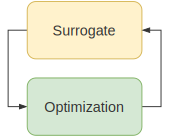
\includegraphics[height=3cm]{content/images/utility/architecture_aso}
                    \caption{Optimization with Simulation-based Iterations (OSI)}
                    \label{fig:surr_opt_architecture_aso}
                \end{subfigure} 
                \begin{subfigure}{0.45\textwidth}
                    \centering
                    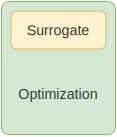
\includegraphics[height=3cm]{content/images/utility/architecture_iso}
                    \caption{Alternate Simulation-Optimization (ASO)}
                    \label{fig:surr_opt_architecture_iso}
                \end{subfigure} 
            \end{subfigure} 

            \caption[Example of a possible combination the optimization algorithm with the surrogate model.]{Example of a possible combination the optimization algorithm with the surrogate model \cite{FigueiraA14}. }
            \label{fig:surr_opt_architecture}    
        \end{figure}


        Almost all related works of parameter tuning could be categorized as \gls{smbo}\cite{JonesSW98}.
        The general \gls{smbo} looks as follows (Figure \ref{fig:sequential_mbo}):
        \begin{enumerate}
            \item The initial sample plan of evaluation points
            \item Build a regression model to provide a hypothesis on the relation between parameters and objectives
            \item Use the build surrogate model as a parameter for optimization strategy. The solutions from the optimization algorithm are a new promising point for evaluation.
            \item Evaluate the new predicted point and add it to the existing samples.
            \item If stop criteria are not met, repeat optimization with the updated samples set.
        \end{enumerate}
        We will present the overview of available works for model-based multi-objective optimization. We will begin with the overview of the project for model-based optimization (mlrMBO) and continue with related algorithms including various optimization improvements.
                                                                                                    % ! We begin with

        % ==== Sequential MBO
        \begin{figure}
            \centering 
            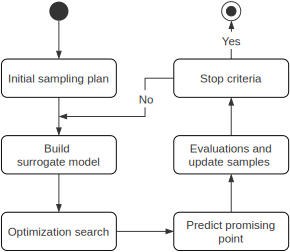
\includegraphics[width=8cm]{content/images/utility/sequential_mbo}
            \caption[General Sequential model-based optimization]{General Sequential model-based optimization (\Gls{smbo})} 
            \label{fig:sequential_mbo} 
        \end{figure}

        % Note that this approach means that

    % --------------------------------------------------------------------------------------------
    % ------------------------------------------------          Approaches
    % --------------------------------------------------------------------------------------------

    % ------------------------------------------------          Frameworks / Platforms
    \section{Platforms and frameworks}
        There are a lot of different projects which can perform multi-objective optimization. Frameworks provide multiple multi-objective algorithms, performance metrics, build-in test problems and extra tools such as plotting and benchmarks. Some frameworks focus on efficient calculations and parallelization\cite{francesco_biscani_2019}, other on implementation of the modern multi-objective algorithms \cite{benitezhidalgo2019jmetalpy, TianPlatEMO} and on support of plenty model-based optimization algorithms \cite{BischlmlrMBO}.

        % ----------------         mlrMBO
        \paragraph{mlrMBO}\cite{BischlmlrMBO} is a modular framework for model-based optimization of expensive black-box functions. MlrBO extends the \gls{smbo} procedure to a multi-objective problem with mixed and hierarchical parameter spaces. Modular structure and integration with \emph{mlr}\footnote{{mlr}: Machine Learning in R. https://mlr.mlr-org.com/} library allows all regression models to be used and compositional techniques such as bagging and ensembling to be applied. Authors implemented 4 different model-based multi-objective algorithms which are distinguished in 3 classes: 1) Scalarization based algorithms that optimize a scalarize version of the black-box functions (\hyperref[alg:ParEGO]{ParEGO}). 2) Pareto based algorithms that build individual models for each objective and complete multi-objective optimization (MSPOT \cite{ZaeffererBNWE13}). 3) Direct indicator based algorithms which also fit individual models, but perform a single objective optimization on an aggregation of all models (SMS-EGO \cite{inproceedings}, $\epsilon$-EGO \cite{WagEGOe}).
        Special features of their framework are multi-point proposal prediction on each iteration. However, it does not provide a combination of different surrogate models into one model.
       
        % ?General characteristics are that they have multiple algorithms on each type of optimization and additional features that they provide. Usually, a surrogate model is predefine and injected into some algorithm for decision making.

        % ----------------         BRISE 2.0
        \paragraph{BRISE 2.0}\label{alg:BRISE} \cite{Pukhkaiev19} is a software product line for parameter tuning. The core topics of their approach are extensibility and variability with the key features such as 1) A \emph{repeater} which automatically decides on the number of repetitions needed to obtain the required accuracy for each configuration. 2) \emph{Stop condition} which validates a solution received from the model and decides, whether to stop the experiment. 3) Connection of a sampling plan and a model prediction validity which provides a \emph{flexible sampling plan}. The main advantage of this sampling plan is that it requires less initial knowledge about the optimization problem.
        Extrapolation model for parameter prediction is exchangeable and it combines surrogate and optimization strategies in each implementation. Several general models, such as polynomial regression surrogate with local search and Bayesian optimization with bandit-based methods strategy(BOHB \cite{FalknerBOHB}), are implemented.  However, the models lack variability and should be designed from scratch for a new domain-problem.

        % ----------------         SMAC
        \paragraph{SMAC} Sequential Model-based Algorithm Configuration (SMAC)\cite{HutterHL11, smac-2017} is a framework for parameter tuning with Bayesian Optimization in combination with a simple racing mechanism on the instances to decide which of two configurations performs better.
        SMAC adopted a random forest model and Expected Improvement (EI) to model a conditional probability. It applies a local search with several starting points to picks configurations with a maximal value of EI. These points improve the exploration possibilities of SMAC in the search space with higher uncertainty and an optimal value of the objective mean. 
        An interesting feature of SMAC is the support of the termination of unfavourable evaluations which are slowing down the optimization process. However, SMAC is limited to a single-criteria optimization and uses a predefined sampling plan.

        % ----------------         Hypermapper
        \paragraph{Hypermapper 2.0} Luigi Nardi et al. \cite{nardi2019practical} presented a multi-objective black-box optimization framework that solves a complex parameter tuning problem with the mixture search space, expensive evaluation and feasibility constrain.
        The proposed approach could be classified as direct indicator based algorithms with constraints validation. During this type of optimization, several identical individual models for each objective are builded and then the single objective optimization on aggregation from all these models is performed. Authors went further and extended this idea to predict no feasible configurations with the extra surrogate model.
        
        The Hypermapper 2.0 are based on a surrogate on a random forest which combines several weak regressors on a subset of samples to yield accurate regression and effective classification models. After scalarizing values from models, Bayesian optimization (BO) method to find an optimal value was applied. Since using only one weight vector would only find one point on the Pareto-optimal front, the weight vector is chosen randomly at each iteration, ensuring that multiple points on the Pareto-optimal front are found. The key features of this approach are the possibility to use prior knowledge, support real variables, feasibility prediction and an excellent final adaptation of the implementation to embedded devices. For explored benchmarks the authors reported that HyperMapper 2.0 provides better Pareto fronts corresponded to state-of-the-art baselines, with better i.e. competitive quality and with considerable saving evaluation budget.
        

    % ------------------------------------------------          Algorithms
    \section{Model-based multi-objective algorithms}
        Fixed optimization components can make general optimization ineffective in the presence of changeable problems. Surrogate construction methodology or even MO algorithm could change to a rich solution closest to real Pareto-optimal frontier.

        % ----------------         ParEGO
        \paragraph{ParEGO}\label{alg:ParEGO} is a scalarization based multi-objective algorithm \cite{Knowles06}. The classical single-objective algorithm \gls{ego} \cite{JonesSW98} of Jones et al. was extended to a multi-point proposal by repeating the algorithm several times with randomly change scalarization weights in each iteration.  The idea of this algorithm is based on Kriging(Gaussian process regression) model and multiple single objective optimization processes on scalarized objectives guaranteeing that multiple points on the Pareto-optimal front could be in prediction. This algorithm and its modification are implemented in mlrMBO\cite{BischlmlrMBO}.


        % ----------------         Distributed Surrogates
        \paragraph{An Evolutionary Algorithm with Spatially Distributed Surrogates} Amitay et al.,\cite{DistrSurr} presented an evolutionary algorithm with spatially distributed surrogates (EASDS). Surrogate models use Radial Basis Function Networks, periodically validating and updating for each partition from samplings points. This generates a complex ensemble surrogate with approximations in local partitions of search space. Spatially Distributed Surrogate models are created for all objectives and then evaluated by NSGA-II \cite{DistrSurr}. The authors describe that their approach achieves better results than single global surrogate models showing an advantage of using multiple surrogates. However, the authors evaluated their algorithm only on bi-objective problems.

        % ----------------         Hybrid surrogate
        \paragraph{A hybrid surrogate-based approach for evolutionary multi-objective optimization} Rosales-Pérez et al.,\cite{HybridSurrRCG} proposed an approach based on an ensemble of Support Vector Machines. The authors describe a model selection process or hyperparameters selection of SVM based on a validation technique and a further injection to the surrogate ensemble. Incremental development of the ensemble includes new information obtained during the optimization and old evidence stores in previous models. 
        The training of a new model represents the SVM grid search in order to find a kernel with the least expected generalization error. This paper presents a model selection process for determining the hyperparameters for each SVM in the ensemble.


        % ----------------         Hierarchical surrogates
        \paragraph{Evolutionary optimization with hierarchical surrogates} Xiaofen Lu et al. \cite{LuST19} apply different surrogate modelling techniques based on motivation on optimization expensive black-box function without any prior knowledge of a problem. They used a pre-specified set of models to construct hierarchical surrogate during optimization. Also, for verification of a surrogate used general accuracy of the high-level model was used. The whole process of the proposed method is about splitting of the accumulated training samples and model-based optimization, which means that the sample plan is static and requires prior information about the problem. 

        Authors show that the hierarchical surrogate structure can be beneficial when the accuracy of the high-level model is larger than 0.5. There with, they noticed that one modelling technique might perform differently on different problem landscapes. Which motivate us to use a pre-specified set of modelling techniques (portfolio with surrogates).
        
        % ----------------         Local search in parallel surrogates 
        \paragraph{Population-based Parallel Surrogate Search} Akhtar et al.,\cite{akhtar2019efficient} introduce a multi-objective optimization algorithm for expensive functions which connect iteratively updated several surrogates of the objective functions. The feature of this algorithm is a high optimization for parallel computation and stacking predictions from the set of Radial Basis Function (RBF) models. The algorithm combines RBF composition surrogate, Tabu, and local search around multiple points. 
        % The authors present an algorithm that can theoretically be applicable to high-dimensional spaces and many-objective problems because the selected surrogate and optimization algorithm are well scalable.


        % ----------------         GALE
        \paragraph{GALE: Geometric Active Learning for Search-Based Software Engineering} Krall et al.,\cite{KrallMD15} developed an algorithm which uses principal components analysis (PCA) and active learning techniques to step-by-step approximation and evaluating of the most informative solutions. Authors notice that MOEAs are not suitable for expensive multi-objective problem because they push a set of solutions towards an outer surface of better candidates which cost many function evaluations. The fundamental idea of the proposed approach is from a large number of solutions to choice more informative ones. Dividing functional landscape into smaller regions and evaluate only the most informative samples from the region. As a result of division of the functional landscape into smaller regions, the function evaluations are saved since only a few the most informative points from the region are evaluated. A drawback of this approach lay in static implementation with MOEA/D.     


        % ===== TABLE
    \begin{table}[]
        \centering
        \caption{The comparison of related approaches. The component behaviour: S - static, V - variability, E-extensibility, D - dynamic}
        \label{tab:my-table}
        \resizebox{\textwidth}{!}{%
        \begin{tabular}{@{}|l|c|c|c|c|c|c|c|c|@{}}
        \toprule
        \multicolumn{1}{|c|}{\multirow{2}{*}{Approach}} &
        \multirow{2}{*}{Multi-objective} &
        \multirow{2}{*}{Sampling plan} &
        \multicolumn{2}{c|}{Surrogate} &
        \multirow{2}{*}{Optimization} &
        \multirow{2}{*}{\begin{tabular}[c]{@{}c@{}}Mixed \\ search space\end{tabular}} &
        \multirow{2}{*}{\begin{tabular}[c]{@{}c@{}}Multi-point \\ proposal\end{tabular}} &
        \multirow{2}{*}{Scalability} \\ \cmidrule(lr){4-5}
        \multicolumn{1}{|c|}{} &
        &
        &
        \begin{tabular}[c]{@{}c@{}}Extrapolation \\ models\end{tabular} &
        \begin{tabular}[c]{@{}c@{}}Composition \\ strategy\end{tabular} &
        &
        &
        &
        \\ \midrule
        mlrMBO\cite{BischlmlrMBO} &
        \cmark &
        static &
        E &
        \multicolumn{2}{c|}{V} &
        \cmark &
        \cmark &
        \cmark \\ \midrule
        BRISE 2.0 \cite{Pukhkaiev19} &
        \xmark &
        flexible &
        \multicolumn{3}{c|}{V} &
        \cmark &
        \cmark &
        \cmark \\ \midrule
        SMAC \cite{HutterHL11}&
        \xmark &
        static &
        S &
        S &
        S &
        \cmark &
        \xmark &
        \cmark \\ \midrule
        Hypermapper 2.0 \cite{nardi2019practical} &
        \cmark &
        flexible &
        S &
        S &
        S &
        \cmark &
        \xmark &
        \cmark \\ \midrule
        ParEGO \cite{Knowles06} &
        \cmark &
        static &
        S &
        S &
        S &
        \xmark &
        \xmark &
        \cmark \\ \midrule
        \begin{tabular}[c]{@{}l@{}}Distributed Surrogates, \\ EASDS \cite{DistrSurr}\end{tabular} &
        \cmark &
        static &
        S &
        E &
        S &
        \xmark &
        possible &
        \xmark \\ \midrule
        Hybrid surrogate \cite{HybridSurrRCG} &
        \cmark &
        static &
        S &
        E+D &
        V &
        \xmark &
        possible &
        \cmark \\ \midrule
        Hierarchical surrogates \cite{LuST19}&
        \xmark &
        static &
        E &
        V &
        V &
        \xmark &
        possible &
        \xmark \\ \midrule
        \begin{tabular}[c]{@{}l@{}}Parallel surrogates, \\ MOPLS \cite{akhtar2019efficient}\end{tabular} &
        \cmark &
        static &
        S &
        E &
        S &
        \xmark &
        \cmark &
        \xmark \\ \midrule
        GALE \cite{KrallMD15}&
        \cmark &
        static &
        S &
        E &
        S &
        \cmark &
        possible &
        \cmark \\ \bottomrule
        \end{tabular}%
        }
        \end{table}

    % --------------------------------------------------------------------------------------------
    % ------------------------------------------------          Conclusions
    % --------------------------------------------------------------------------------------------
    \section{Conclusions}

        As shown before, surrogate or model-based optimization suites for an expensive black-box problem. The summary of the related work is given in Table \ref{tab:my-table}. Nevertheless, this approach also has open questions and limitations:
        \begin{itemize}
            \item Multi-objective hypothesis. A \emph{limited amount} of surrogate models can handle 
            only with a limited dimensions of parameter and objectives. Scaling is an open research question for existing multi-output surrogate models.
            \item \emph{Surrogate is domain-specific.} to improving and to reach the best prediction, we should know the objective surface in order to apply a specific surrogate. Universal surrogates can gain optimal results but not the most reliable \cite{abs181207958, LuST19}.
            \item The quality of prediction depends on \emph{how many samples} we make for a specific type of surrogate. There is a trade-off between reduction of a sample size and maximization of a quality of prediction. Overfitting, as well as underfitting, can guide optimization in a wrong direction.
            \item Often an optimization algorithm and surrogate model are \emph{coupled} extremely tightly. This dependence on one another makes the general approach biased against specific problems. Reimplementing these algorithms for each usage scenario becomes timeconsuming and error-prone. 
        \end{itemize}

        To our knowledge, there are no researches which studie complex combinations of a surrogate model and their impact on a solution quality. After the analysis of the related work, we can define research gaps such as:
        \begin{description}
            \item[Surogate combination] Previous researches have shown that the selection of the surrogate model can profoundly affect the quality of the optimization solution. Furthermore, they mention that the surrogate is domain-specific, and the same technique might perform differently on different problems \cite{LuST19, HybridSurrRCG}. The overall research gaps of the surrogate model's flexibility might be divided into the following subproblems:
            \begin{enumerate}
                \item The dynamic combination of different single-criteria models is crucial to solve the multicriteria problem. It must be feasible to substitute the type of nested surrogate model for an arbitrary criterion component. This could provide higher variability for the surrogate model to describe arbitrary optimization problems. Therefore, the technology which allows the surrogate compositional model to be established is necessary.
                \item The investigated works conclude that variants in the choice of the model improve the final result. Unfortunately, most authors used only one type of the model with various hyperparameters. Therefore, there is a necessity for a portfolio with surrogate models.
            \end{enumerate}
            \item[Sampling plan] A static plan requires additional knowledge of the surface of the problem, which is usually not possible to obtain. Moreover, arbitrary decisions of the sample size might be a reason which leads to inaccurate models and further wrong results. This problem may occur because the surrogate model might be overfited or underfited, and the result is a waste of samples and resources. 
        \end{description}

        % --------------------------------------- Scope of work
        \subsection{Scope of work}
        In this thesis, we focus on the improvement of the surrogate models for the multi-objective problem. Surrogate-based optimization has proven its effectiveness in many areas of engineering and in applications where data is expensive or difficult to evaluate. While other methods also exist, we select \gls{moea} as the main solver because it can be applied to a wide range of problems and because it gives a broad understanding of how Pareto-front might look. The problem type is expensive, multi-objective, derivative-free/black-box system without constraints.

        Design gap in optimization and parameter tuning lays in the quality of the surrogate model:
            \begin{itemize} % ! refries
                \item Select proper surrogate model 
                \item Surrogate composition for multi-dimensional space
                \item Sampling strategy
                \item Surrogate validation
            \end{itemize}

        \paragraph{Goals:}
        \begin{enumerate}
            \item Find diverse solutions with minimal distance to real Pareto frontier.
            \item Reduce the evaluation budget.
            \item Develop modular and extensible architecture that could be combined with other frameworks. 
            \item Improve the backward computationally with the single-objective parameter tuning.
        \end{enumerate}

        % Also optimization and composition of multi-objective solvers is a rapidly expanding area of research and a full survey of that work is beyond the scope of this thesis.



        % --------------------------------------------------------------------------
        % Fixed components can make the optimization of changeable problems ineffective. 
        % Appropriate surrogate construction methodology or combination of multiple solving algorithms could improve the final solution. The significant works analyze that compositional architecture with several surrogate models is a promising direction to improve the multi-objective solution. 
        % Moreover, almost none of the approaches examined the size of the surrogate sample set. 

        % !There is a clear need for a method to provide and distribute ready-to-use implementations of optimization methods and ready-to-use benchmark and real-world problems. These modules should be freely combinable. Since the above mentioned issues are not constrained to evolutionary optimization a candidate surrogates solution should be applicable to a broader range of search algorithms



        % However, it lacks fundamental features that makes it ineffective in the presence of applications with non-feasible designs and prior knowledge.


        % Our work is similar in nature to the approaches adopted in the Bayesian optimization literature [27]. Example of widely used mono-objective Bayesian DFO software are SMAC [15], SpearMint [30], [31] and the work on tree-structured Parzen estimator (TPE) [6]. In particular, the use of a full Bayesian ap- proach will help to leverage the prior knowledge by computing a posterior distribution. Exploration of additional methods to warm-up the search from the design of experiments literature

        % \paragraph{Hyperopt}




        % Based on a survey\cite{SoftSurvey} there still exist such as:
        % \begin{itemize}
        %     \item 
        % \end{itemize}


        % Some features of their approach are 


        % We extend the idea of stochastic RBF to be suitable for the algorithm configuration task. It is a model-based algorithm that cycles from emphasis on the objective to emphasis on the distance using a weighting strategy. 
        
        % The main advantage of LHS is that it does not require an increased initial population size for more dimensions.


        % exploration, exploitation and diversification during each algorithm iteration.


        % To our knowledge, there exists no research that investigates how deep networks affect the performance of surrogate-assisted multi-objective evolutionary algorithms. If neural networks were used, the approaches usually adopted only one hidden layer. Additionally, we can also see that there exists a multitude of ways a surrogate model can be integrated into an evolutionary algorithm

        % Previous studies have shown that the choice of modeling technique can highly affect the performance of the surrogate model-assisted evolutionary search.

        % However, one modeling technique might perform differently on different problem landscapes. Without


        % OpenTuner is different from our work in a number of ways. First, our work supports multi-objective optimization. Second, our white-box model-based approach enables the user to understand the results while learning from them. Third, our approach is able to consider unknown feasibility constraints. Lastly, our framework has the ability to inject prior knowledge into the search. The first point in particular does not allow a direct performance comparison of the two tools.

        % over the entire space would result in a waste of samples.


        % This is especially the case for a SMBO

        % The black-box function can be more complex, for example a machine learning pipeline which includes preprocessing, feature selection and model selection.


        % Consequently, the advantage of the multi-objective candidate generation to produce a set instead of single points is not only used for improving the exploration of the decision space, but also for obtaining a well-spread batch of solutions.


        % For example, OEGADO \cite{ChafekarSRX05} creates a surrogate model for each of the objectives. The best solutions in every objective get also approximated on other objectives, which helps with finding trade-off individuals. The best individuals are then exactly evaluated and used to update the models.


        % ? Bayesian optimization (BO) methods often rely on the assumption that the objective function is well-behaved, but in practice, the objective functions are seldom well-behaved even if noise-free observations can be collected. In \cite{bodin2019modulating} propose robust surrogate models to address the issue by focusing on the well-behaved structure informative for search while ignoring detrimental structure that is challenging to model data efficiently.
    \chapter{Concept}\label{sec:concept}

    \begin{blockquote}
        \paragraph{Intent:} General reminder and answer of RQ's
        
        Structure:
        \begin{description}
            \item[1. Surrogates models combinations] Surrogate model is not universal. Domain-specific $\rightarrow$ Surrogate model portfolio 
                \begin{enumerate}
                    \item Surrogate model is not universal. Domain-specific $\rightarrow$ \textbf{Surrogate model portfolio}
                    \item Objectives have different complexity surface $\rightarrow$ Surrogate model is not universal $\rightarrow$ Describe objectives independently. \textbf{Heterogeneous/Composition surrogate model} 
                \end{enumerate}
                  
            \item[2. Dynamic sampling plan] Use sampling plan while surrogate is not valid
                \begin{enumerate}
                    \item Surrogate Validation. Stages and thresholds
                    \item Metrics
                \end{enumerate}

            \item[3. Scalability] Compositional surrogates in many-objective space
                \begin{enumerate}
                    \item Problem: Random solver on high dimensional space $\rightarrow$ Solution: Light surrogates 
                    \item Solving problem in subset of dimensions
                    \item Categorical parameters*
                \end{enumerate}

            \item[4. Discussion] General Conclusions. Infill criteria for Pareto-optimal solutions
        \end{description}
    \end{blockquote}

    \epigraph{``All models are wrong but some are useful``}{\textit{– George Box}}

    This section presented a general idea of the improvement in the surrogate-based optimization for black-box function. 

    % Mainly two groups are affected by this problem:
    % \begin{itemize}
    %     \item Application engineers who need to choose, implement, and apply state-of-the-art algorithms without in-depth programming knowledge and expertise in the optimization domain
    %     \item Developers of optimization methods who want to evaluate algorithms on different test problems and compare a variety of competing methods
    % \end{itemize}

    The usual problem is a trade-off in producing the best possible multi-objective solution with less effort. Because we consider system expensive to evaluate, an effort first of all means evaluated examples. Each of these evaluations can require much time, energy, or other resources. That is why the main comparison criteria for the approach is solving the multi-objective problem with a limited evaluation budget. %! change quality to count 

    In this work, under solving a multi-objective problem, we intend to find a set of none-dominated points that cover a wide range of objectives values and close as possible to real Pareto front. Multiple algorithms could be applied, but MOEA is the favored choice. The advantage of evolutionary algorithms is that it could be easily modified. It operates on a set of solutions candidates, that are well-fitted to approximate Pareto-front. Finally, evolutionary algorithms can estimate highly complex problems in various use-cases. 

    If evaluations of the problem are expensive, the real count of experiments could be reduced throw applying a multi-objective algorithm on a surrogate model. This technique is the preferred choice for functional optimization when the evaluation cost is high.

    As shown before, surrogate or model-based optimization suited for an expensive black-box problem. Nevertheless, this approach also has open questions and limitations:
    \begin{itemize}
        \item \emph{Surrogate is domain-specific.} For improving and reach the best of the best prediction, we should know in cross-grain underlying objective surface to apply specific surrogate. Universal surrogates can gain optimal results but not the most reliable possible \cite{abs181207958, LuST19}.
        \item Multi-objective hypothesis. A \emph{limited amount} of surrogate models can handle multi-dimensional parameter space. Also, scaling is an open research question for existing multi-output surrogate models.
        \item Quality of prediction depends on \emph{how much samples} do we have for a specific type of surrogate. There is a trade-off between reducing sample size and maximize the quality of prediction. Overfitting, as well as Underfitting, can guide optimization in the wrong direction.
        \item Multi-objective optimizations with \emph{categorical features} are standard in engineering practices. Parameter tuning with that type of space is not trivial.
        \item Often Optimization algorithm and surrogate model are very \emph{tightly coupled}. Profoundly connected implementation suitable for a specific type of problem and require prior knowledge about a problem. Reimplementing these algorithms for each usage scenario becomes timeconsuming and error-prone.
    \end{itemize}

    
    %? The main objective of this part is to provide a thorough treatment of multi-objective parameter tuning with evolutionary algorithm(s)


    % The solution techniques and parametric selections however are usually problem-specific. \cite{abs181207958}
    % --------------------------------------------------------------------------------------------
    % ------------------------------------------------     RG1: Models combinations     
    % --------------------------------------------------------------------------------------------

    \section{Surrogates models combinations \ref{RQ1}}

        This general topic introduces compositional surrogate as a proxy model that approximates objectives surface and supports MOEA to evaluates near a multi-objective solution and predict better multi-objective samples on each iteration.

        % ------------------------------------------------     Compositional model       
        \subsection{Compositional Surrogate Model}
            There is a typical strategy to combine several instances of surrogate models to create a complex hypothesis (surrogate). Usually, authors present a sophisticated design that uses one type of model for each objective or subproblems. Nonetheless, the surrogate model is not universal to describe objectives independently. 

            The perspective way to create multi-objective surrogate is stacking multiple simple models into one that describes complex objective space. Notwithstanding that those models could be completely different and build in parallel, they still related because fitted on intersection features.
            Splitting optimization problem to multiple stages improves the reusability of code and makes approach scalable. Nevertheless, we can switch from single-obj to multi obj and change optimization technic on the fly.

            The concept of the compositional model means a combination of a heterogeneous surrogate model that looks uniformly for the optimization algorithm. So it is possible to extend single-criteria models for multi-criteria tasks and dynamically reconstruct problem representation from mixed model parts. In this thesis, the compositional model means a surrogate model that combines various surrogates models for each optimization objective.

            The concept of the compositional model means a combination of a heterogeneous surrogate model that looks uniformly for the optimization algorithm. So it is possible to extend single-criteria models for multi-criteria tasks and dynamically reconstruct problem representation from mixed model parts. In this thesis, the compositional model means a surrogate model that combines various surrogates models for each optimization objective: horizontal variability, flat surrogate combination. 
            That approach should be capable, outperform other algorithms with static models on a real black-box problem with the unknown objective surface. On the other hand, the user could inject his domain knowledge as a combination of surrogate models. 



        
        % ------------------------------------------------     Portfolio      
        \subsection{Surrogate model portfolio}

            \paragraph{Domain-specific problem} With gain to find the best solution with less effort surrogate models is domain-specific. It's mean that from two surrogate models in two different problems the best surrogate is changing. It could interpreter as Non-free lunch theorem in model-based optimization. If we extend this argument then the same optimization problem in different parameter tuning iteration could be interpreted as another optimization problem. This means that to reduce effort and increase the convergence of an algorithm we should change the surrogate model depend on how much samples do we have. As one would expect, no approximation method is universal. This leads us to use a portfolio with surrogate models. As a negative consequence, the model fitting additional introduces an additional overhead into the optimization

            With the flexibility that provides a compositional system to combine several models, that is valuable to produce several variants of compositions from available surrogates. This functionality requires validation criteria to discard those that are not valid and comparison metrics to range and combine the best ones. Many hooks are created to combine and solve surrogates models. This gives flexibility to the combination of hypotheses, testing, and solving/optimization. Bagging or ensemble technique can be applied to both: the surrogate models and the optimization algorithms.

            Besides, it grates motivation to use the latest state-of-the-art algorithms together because the modular structure of the compositional model and portfolio it is a skeleton for optimization. 


        % ------------------------------------------------     RG1.1: Scalability     
        \subsection{Scalability \ref{RQ1.1}}
            Besides the surrogate composition, there is an open sub-question of how to scale this approach. Surrogate model and optimization algorithm suffer from this.

            % -------------------------     Many-objective      
            \paragraph{Many-objective compositional surrogates}
            Problem: Random solver on high dimensional space $\rightarrow$ Solution: Light surrogates 


            \paragraph{Marginal sub-problem on high dimensions}
            Solving problem in subset of dimensions

            % -------------------------     Categorical parameters      
        \subsection{Categorical parameters}

        Feature encoding is used to support a categorical parameter for generic models. Coding features for a surrogate model can transform those in a meaningful form, understandable for a surrogate model. Encoding represents a feature in an alternative form that helps model instantiation relation and a correlation between features. Based on this inner interpretation model can predict the values of labels based on a parameter vector. The problem occurs in reverse interpretation of these optimal predictions in the context of parameter space. Often a found solution is not a feasible point from parameters space. As a possible solution, it partly transforms problems in multiple classification tasks and then considers there relation as optimization with continuous probability [TPE]. For the general surrogate model with mixed parameters, we can solve a problem orthogonally with multiple optimizers. All samples with the categorical feature are encoded and fitted to the surrogate models. Then we use this model as an optimization target.  We incrementally solve this optimization problem on a subset of dimensions. For example, we find optimal parameters in categorical dimensions with local search and then fix these values and optimize surrogate on the left subset of numerical dimensions where categories are fixed. 




    % --------------------------------------------------------------------------------------------
    % ------------------------------------------------     RG2: Sampling plan     
    \section{Sampling plan \ref{RQ2}}
        For expensive optimization problems, it would be useful to modulate a problem using quite a small number of most informative examples. Nonetheless, almost sequential model-based approaches use a static sampling plan. If the oracle does not determine the required number of samples, it can be done dynamically based on the quality of the surrogates. 

        % -------------------------     Surrogate Validation      
        \subsection{Surrogate Validation}
        It is necessary to sacrifice a small portion of the data experiments to check the quality of the surrogate model on it. Based on validation results, we can discard inadequate models and elaborate evaluate the solutions from valid models. If neither model is valid, this means that the best solution right now is a solution from the sampling plan. This process will be repeated until a complete, valid surrogate model is obtained.
        In the context of parameter tuning, evaluation surrogate validity based only on the coefficient of determination(R2) metrics is incorrect. A common misconception lay in prefer global accuracy score over the score in the optimal region. That is why evaluation surrogate validity based only on the coefficient of determination(R2) metrics is incorrect\cite{nardi2019practical}. Global R2 can be anyway used as a threshold for exceeding which the model becomes not valid even with additional estimations.  

                                            [-- Fig:1   decisions in model validation   --]

        The central concept for surrogate validation lay in adaptation best practices from the machine-learning community for evaluation estimator performance.  
        With the sequential selection of a model, there is a risk of overfitting on the test set because the instances can be calibrated until models perform optimally. It means that the test set 'leak' to train set and final metrics does not report on the generalization performance of surrogate. Deal with this problem, yet another portion of samples can handle as a so-called 'validation set.' In that set, surrogates passed validation on global metrics, and when the evidence seems to be successful, final evaluation performs on the test set. Final metrics show accuracy on the interested search space (none-dominated solution from test set).

        The decision on which surrogate model is better made based on the metrics from all stages.  If the model does not have a sufficient threshold, it is rejected as not valid. If there is no valid model, the assumption of the next configuration is accepted from the sapling plan.

        In order to generalize well, it is crucial that your training data be representative of the new cases you want to generalize to.


        % -------------------------     Metrics      
        \subsection{Metrics validity for optimization}
        Validation accuracy threshold for general search space and non-dominated region

        Models are validated in two stages. The first stage estimates the overall surrogate accuracy. If it is more than a certain threshold, then the model goes to the next step. it evaluates the accuracy of the model already on a new set of data that characterize the area of interest in optimization.


        % overfit - underfit
    
        % metrics comparison


    % --------------------------------------------------------------------------------------------


    % --------------------------------------------------------------------------------------------
    % -----------------------------------------------------       Discussion      ----------------
    % --------------------------------------------------------------------------------------------
    \section{Discussion}

        In this thesis, proposed approach for combination surrogates for multi-objective optimization and dynamic sampling plan based on surrogate validation.

        % -----------------------------------------------------       Infill criteria       ------
        \paragraph{}{Infill criteria}
        In the case of MOEA, solution of algorithm present as non-dominated final population. Based on unbiased, multi-objective criteria, they all uniformly could be presented as a prediction to the next evaluation. They represents current solution based on the surrogate model. Nevertheless, there is prior knowledge available in samples which can be taken into account. To reduce the number of candidates in the population, it is possible to deny those in which the distance to the nearest available sample is less than their average distance.
        So there are two strategies for predicting from a population:
        \begin{itemize}
            \item Prior and posterior knowledge. Based on changing metrics in available and proposed solutions
            \item Posterior knowledge. Proposed solutions are all equal
        \end{itemize}


        
        % -----------------------------------------------------       Conclusions       ------
        Also, to the best of our knowledge, has not been previously or stingy reported in the efficient multi-objective optimization.
        Contribution:
        \begin{itemize}
            \item Surrogate combination/composition with heterogeneous models
                \begin{itemize}
                    \item Surrogate models portfolio
                    \item Compositional surrogate model
                    \item Combination of different(orthogonal) solvers
                \end{itemize}
            \item Surrogate portfolio. Search a better hypothesis  for a specific problem at a particular stage of parameter tuning
            \item Metric combination for evaluation Pareto optimal points
            \item Samples size depends on model(s) validity
            \item Concepts
                \begin{itemize}
                    \item Combination of different(orthogonal) solvers
                    \item Infill criteria for prediction selection
                \end{itemize}
        \end{itemize}

        We argue that the proposed concept from this thesis is the preferred choice for functional optimization when the evaluation cost is large.


        % structures include more than one possibility, as described above. Nevertheless, this level

        % Finally, another aspect worth mentioning is the fact that GSM appears in more than one cell. Indeed, hybrid methods


        % where the algorithms are allowed to query an oracle for additional data to infer better statistical models


        % They also reported that a speedup of a factor of 10 can nevertheless be obtained.
    \chapter{Implementation}

\begin{blockquote}
    \paragraph{Intent:} Details of implementation. Requirements: reusable components, unify interfaces. Duck typing 
    
    Structure:
    \begin{description}

        \item[1. Compositional surrogate model] heterogeneous model combination on each objective
        \begin{enumerate}
            \item Model-union class. Stacking surrogate. Tree composition
        \end{enumerate}

        \item[2. Surrogates validation] When the surrogate model can be helpful?
        \begin{enumerate}
            \item Validation workflow. Adaptation from Data science
            \item Hypothesis portfolio validation and combination
            \item Stages and thresholds
        \end{enumerate}

        \item[3. Solvers] Optimization algorithms. Solve problem based on surrogate model(s)
    \end{description}
\end{blockquote}
% ================================================================================================

This section describes the details and decisions in the implementation of the proposed thesis concept. Implementation should be flexible and usable. Consist of buildings blocks with consistent interfaces. Achieve a wide diversity of solving problems within extension from other algorithms and frameworks. Based on best practice \cite{buitinck2013api}, the implementation accepts the following principles:
\begin{itemize}
    \item \textbf{Components.} Simple and efficient, reusable in various domains. Whenever possible, new functionality is implemented and composed from existing building blocks.
    \item \textbf{Separation of concerns.} Implementations of surrogate models and optimization algorithms are unrelated and interchangeable. 
    \item \textbf{Non-proliferation of classes.} Samples and Datasets are represented as arrays or data frames. Hyper-parameter names and values are represented as standard Python strings or numbers whenever possible. This keeps components easy to use and easy to combine with other libraries \cite{buitinck2013api}.
\end{itemize}


The next dependencies are chosen to achieve the above mention principles:
\begin{description}
    \item \textbf{Scikit-learn} \cite{art-scikit-learn} is one of the most popular machine learning framework that accomplishes with a variety of learning tasks. The critical features are excellent documentation and reusable components in various contexts. Extensibility and consistent interfaces lead that the library has gathered a large community. Scikit-learn integrates well with many other Python libraries. 
    \item \textbf{pygmo2} \cite{francesco_biscani_2019} is efficient parallelization scientific library for local and global optimization. Key features of their project are efficient implementations of bio-inspired and evolutionary algorithms and unified interface to optimization algorithms and problems. 
\end{description}

               



% \paragraph{Reusability in parameter tuning} Parameter tuning can be splitted down into steps that are common for the many/single-objective optimizations. Each step in optimization workflow has variability via implemented interfaces. Single-objective hypotheses can be combined for multi-objective optimization with compositional design. API of metric-learn is compatible with scikit-learn, the leading library for machine learning in Python. This allows to use all the scikit-learn routines (for pipelining, model selection, etc) with metric learning algorithms through a unified interface.


% \paragraph{Inner interfaces} Supervised learning consists in learning the link between two datasets: the observed data X and an external variable y that we are trying to predict, usually called target or labels. Most often, y is a 1D array of length $n samples$. All supervised estimators in scikit-learn implement a fit(X, y) method to fit the model and a predict(X) method that, given unlabeled observations X, returns the predicted labels y. Using arbitrary regression models from scikit-learn as surrogates. Problem that each optimization framework/library use inner interfaces. It is necessary to define a standard that implements best practices for extension libraries \cite{buitinck2013api}. We introduce new Model-based line for parameter tuning. 



% --------------------------------------------------------------------------------------------
% ---------------------------------------------------       Compositional surrogate      
% --------------------------------------------------------------------------------------------
\section{Compositional surrogate}
    Model-union class (Figure \ref{fig:munion}) is a place where several heterogeneous models could be combined. This class is as meta-model that wraps and aggregate estimations from several sub-models. Model-union could be combined in a tree structure with arbitrary models that support require interface. There are two estimation modes:
    \begin{itemize}
        \item \textbf{Stacking.} It is an ensemble learning technique to combine multiple regression models by a meta-regressor. The individual regression models are trained based on the whole training samples. The final label prediction is averaged from all models outputs.
        \item \textbf{Split y.} A straightforward technique to combine several regression models to multi-label prediction. The individual regression models are also trained based on the whole training samples, but final prediction produces from a model's outputs concatenation. For each model features space is common, but labels are orthogonal. This functionality allows as to produce multicriteria compositional models from combinations of single objective models.

    \end{itemize}

    % ==== Sampling plan
    \begin{figure}
        \centering
        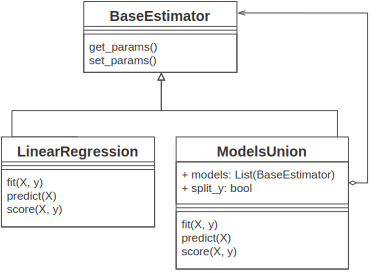
\includegraphics[width=10cm]{content/images/munion_class}
        \caption[Models-union class]{Class diagram of \textit{ModelsUnion}. Scikit-learn tends to use "duck typing", so building a model which supports require methods suffices for compatibility. Internal classes such as \textit{BaseEstimator} provide boilerplate code and is used for clarity and convenience intent.} 
        \label{fig:munion} 
    \end{figure}  

    ModelsUnion class puts the compositional model on one line with other surrogate models. It allows us uniformly validate many surrogate models and combine them in a surrogate portfolio.

% --------------------------------------------------------------------------------------------
% ---------------------------------------------------       Optimization orchestrator     
% --------------------------------------------------------------------------------------------
\section{Optimization orchestrator}
    The \textit{TutorModel} class is the orchestrator of all optimization's processes. It holds a surrogate portfolio, makes validation decisions, combines valid surrogate hypothesis and brings them together with optimization solvers (Figure \ref{fig:tutor_activity}).

    %! [ === Model product line === ]


    % ---------------------------------------------------        Validation
    \subsection{Surrogates validation}
        Each surrogate pass validation in several stages (Figure \ref{fig:simsim_activity_validation}): 1) Surrogate selection based on cross-validation results. In this stage define lower bound for overall accuracy. We notice that pass this threshold does not guarantee that surrogate is useful, but we sure that lower values detect models as useless. By default threshold \#1 defines as R2 less than 0.65. 2) Check accuracy in the region of interest. Finalist models chacks on unseen data to validate extrapolation quality and accuracy in optimal points. By default, R2 at this stage is also should be more than 0.65. Accuracy in optimal points is used for sorting champion models and corresponding solutions. Threshold's values selected from practical and theoretical use.

            % ==== activity_validation
            \begin{figure}
                \centering
                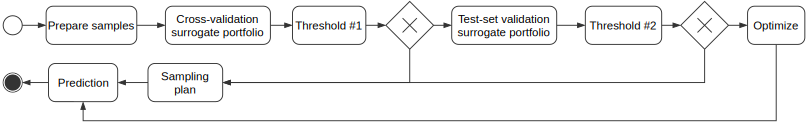
\includegraphics[width=\textwidth]{content/images/simsim_activity_workflow}
                \caption[General workflow activity]{General optimization workflow for model-based optimization iteration with validation in two stages.}
                \label{fig:simsim_activity_validation}
            \end{figure}

        The test set by default is 25\%. On left 75\% used cross-validation in 4 rounds. It means that gained four folds of samples and models training perform in three folds and testing on the fourth fold. It performs results for select or rejects surrogates combinations. After on test set gain information about the quality of possible solutions from surrogate 


    % ---------------------------------------------------        Portfolio        
    \subsection{Hypothesis portfolio}
    In general, surrogate models can be divided into two groups: a multi-output model for all objectives and compositional model with single-output models. All models pass validation equally, but after cross-validation single-objective models should combine in the complex surrogate hypothesis. 
    Ultimately, all objectives should be restored from valid surrogates and if some objective dimension has more models than other, last duplicate themselves to fill a gap. After complete restoring, compositional models with multi-output models validate further on the test set.

    % In the case of mixed surrogates models portfolio, validation pass in two groups: multi-objectives and single objective surrogates. In single-objective surrogates group must additionally restore complite hypotheisis for the multi-dimensional objective surface.

        % ==== Figure
        \begin{figure}
            \centering
            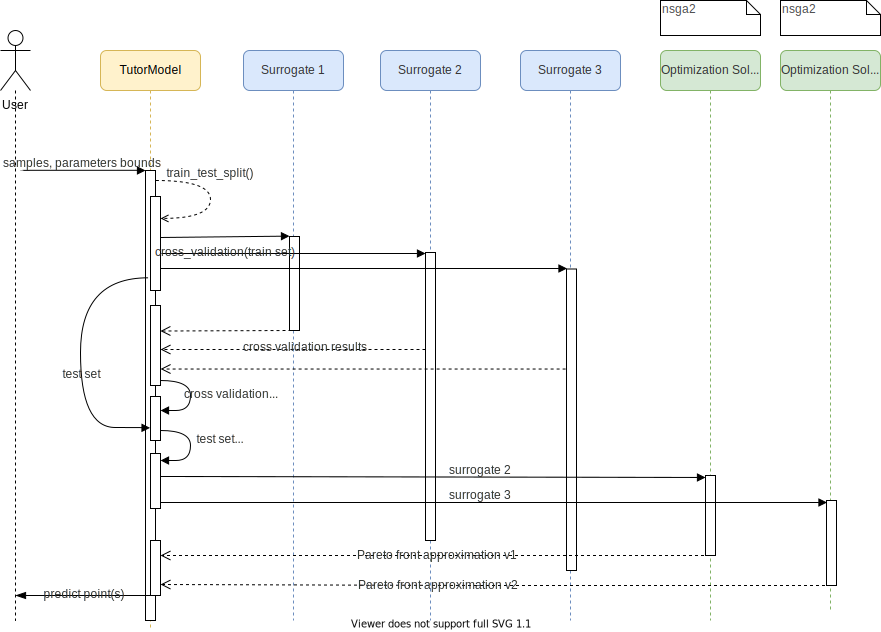
\includegraphics[width=\textwidth]{content/images/portfolio_validation_solv}
            \caption[Portfolio validation activity]{This is a validation and optimization workflow of several surrogates}
            \label{fig:tutor_activity}
        \end{figure}



    % ---------------------------------------------------        Sampling strategy
    \subsection{Sampling strategy} In many practical problems, only a restricted budget is spendable. Each evaluated point should be informative to reduce cost and improve interpolation by models. The most straightforward method of sampling design is a random witch for small sample sizes, that often produce clusters of samples. Conversely, there are also quasi-random distributions that produce informative samples that cover space more evenly. Most popular algoruthms are Sobol\cite{Sobol1999} and Latin hypercube sampling. 
    Out of the box, we provide Sobol sampling and random sampling.
    
    
    % Oversampling and undersampling in data analysis. Alleviate imbalance in the dataset. 
    % Imbalance in dataset is not always a problem, more so for optimization tasks. 

    % The main gain for models not to provide best accuracy on all search space but provide possible optimum regions.
    % Accuracy in prediction optimal regions or points from there will direct the search in the right direction.

    % Predictor variables can legitimately over- or under-sample. 
    % In this case, provided a carefully check that the model assumptions seem valid.

    % for other set of parameters, and make a choice from more diverse pool of models.

% --------------------------------------------------------------------------------------------
% ---------------------------------------------------       Solvers      
% --------------------------------------------------------------------------------------------
\section{Optimization solvers}


    Solvers role is to apply an optimization algorithm on the surrogate and find a solution(s). Most solvers implemented with Multi-objective evolutionary algorithms such as NSGA2, MOEA/D, Multi-objective Ant Colony Optimizer (MACO) or Nondominated Sorting Particle Swarm Optimizer (NSPSO). 
    Specifically added solver with a combination of several multi-objective genetic algorithms with a shared population (MOEA-Ctrl).

    Accordingly, on this step, a version of the solver with a scalarization of surrogates values possible witch optimize with any optimal heuristics. In this case, only one optimal point is obtained from the Pareto front, so the process must be repeated as many times as necessary to obtain the required count. 

    Optimization framework requires the definition of custom problems. Optimization algorithm receives the surrogate model as a parameter and builds custom optimization problem on it. In the case of a genetic algorithm, gain the perspective population of parameters, that could be selected as a Pareto front approximation. If several surrogates valid - several Pareto-front approximations obtain. There are two approaches to select the most informative solutions: 1) select Pareto approximation from surrogate with the highest accuracy in non-dominated points. 2) Assume that all approximations are valid and all points could be selected. In this case, intersection predictions from samples have a higher probability of being selected

    For singl-objective problem was adopted Extended Ant Colony Optimization algorithm (gaco). Feature of this algorithm consist in applying Gausian process regresion to generate future generations of ants. 

    All default solver allgorithms are implemanted in pygmo2 \cite{francesco_biscani_2019}.
    % Optimization algorithms. MOEA. A Python platform\cite{francesco_biscani_2019}  to perform parallel computations of optimisation tasks (global and local) via the asynchronous generalized island model.

    % decorators for single-objective solver with multi-objective surrogate 








% ----------    Designing a Sampling Plan
% \paragraph{Designing a Sampling Plan} The most straightforward way of sampling a design space in a uniform fashion is by \cite{EngSurMod} means of a rectangular grid of points. 
% Random sampling has the downside that for small sample sizes, there is often signficant clustering of samples, which is not ideal for interpolation since clustered samples can be wasteful. Instead, often a better option is to use a Latin hypercube, which enforces a condition that sample bins may not share the same coordinates for any coordinate axis







% Without automated tools, it can take days for experts to review just a few dozen examples.  In that same time, an automatic tool can explore thousands to millions to billions more solutions. People find it an overwhelming task just to certify the correctness of conclusions generated from so many results.


% Managing complex execution Strategies


% The simplifications are mean to discard the superfluous details that are unlikely to generalize to new instances. However, to decide what data to discard and what data to keep, you must make a hypothesis. For example, a linear model makes the hypothesis that the data is fundamentally linear and that the distance between the instances and the straight line is just noise, which can safely be ignored.



% sklearn 'duck typing'. This means that estimators are defined by interface, not by inheritance, where the interface is entirely implicit as far as the programming language is concerned.

% Variants in the evaluation of sets of solutions for each hypothesis. Each hypothesis has quality metrics. Solution(s) from each hypothesis have also own metrics.


% Intuition of why random forest is a good model: •Good at non-linearity, multi-modality and non-smoothness. A decision tree is a non-parametric supervised machine learning method widely used to formalize decision making processes across a variety of fields. The combination of many weak regressors (binary decisions) allows approximating highly non-linear and multi-modal functions with great accuracy. In addition, random forests naturally deal with categorical and ordinal variables which are important in computer systems optimization.

    \chapter{Evaluation}\label{sec:evaluation}


\begin{blockquote}
    \paragraph{Intent:} Performance evaluation 
    Structure:
    \begin{description}

        \item[Experimental setup] Optimization problems types, evaluation assumption and budget, repetition

        \item[Benhmark 1] Default Tutor-model(portfolio, thresholds) on plethora types of multiobjective problems
        \begin{enumerate}
            \item default Tutor-model parameters
            \item surrogate portfolio items
            \item Baseline: MOEA
        \end{enumerate}

        \item[Benhmark 2] Parameter selection of Tutor-model with the dynamic sampling plan
        \begin{enumerate}
            \item Parameters: prediction count, train/test split, stacking solutions. thresholds(x2), solver
            \item Subset of problems
            \item Baseline: Static vs Dynamic. Parameters tune
        \end{enumerate} 

        \item[Benhmark 3] Many-objective optimization. Objectives>10
        \begin{enumerate}
            \item Static Heterogeneous compositional surrogate vs. Homogeneous compositional surrogate
            \item Base line: MOEA or Random
        \end{enumerate}

        \item[Discussion] Results interpretation
    \end{description}
\end{blockquote}


In this section, we present the results obtained for proposed methods on test problems with diverse objective landscape and with a various number of search variables.

% ? MOEA is called globally convergent if the produced, non-dominated population converges to the true Pareto front while the number of generations goes to infinity.

For this study, we did not do extensive parameter tuning: NSGA-II and surrogates were run using their default settings.
\cite{kouwe2018benchmarking}

% --------------------------------------------------------------------------------------------
% ------------------------------------------------     Experimental setup     
% --------------------------------------------------------------------------------------------
\section{Experimental setup}
The measurements were performed on an Intel Core i7-8700CPU machine with 64G of memory using Fedora Server 29.

    % ---------------------------------     Optimization problems
    \subsection{Optimization problems}
    For comparison was selected several widespread synthetic benchmark suites. All of them are scalable in parameters space and some in objective space also. They simulate real life problem and have main related challenges such as multi-modality, different surface type, not uniform search space. All problems assumed global minimization for all objectives.

    The following property \cite{WFGref} could characterize optimization problems:
    \begin{itemize}
        \item Modality is the property of objectives surface. Test problems are either unimodal with one global optimum or multimodal with several local optima. Multimodal problems are more complicated than unimodal problems and more similar to real-world issues.
        \item The geometry of a Pareto optimal surface can directly influence the performance of the algorithm. Problems could be related to inner metrics of algorithms to estimate the dominance in population.
        \item The bias of landscape transformations impacts the search process by biasing the fitness landscape. This property means that uniformly distributed parameters mapping to predisposition area in objective space. This type of problem could be mode difficult if bias region is far away from the Pareto-optimal front.
        \item Many-to-one fitness mapping means that different parameter vector could produce the same objective vector. This property made the search more difficult to optimizers because increase likelihood of that parameters variations do not generate new objective vector.
    \end{itemize}

    % ! [===    Many-to-one, bias, Modality, geometry  ===]
        % -----------------------------  ZDT      
        \paragraph{ZDT} widespread test suite\cite{ZitzlerDT00} was conceived for two-objective problems and takes its name from its authors Zitzler, Deb and Thiele. Each test function involves a particular feature that is known to cause difficulty in the evolutionary optimization process, mainly in converging to the Pareto-optimal front.
        For benchmarks selected following problems:
        \begin{itemize}
            \item ZDT4: function has 21 local Pareto-optimal fronts and therefore is highly multi-modal. Also called multifrontal problems.
            \item ZDT6: function has a non-uniform search space: the Pareto-optimal solutions are non-uniformly distributed along the global Pareto front, and also the density of the solutions is lowest near the Pareto optimal front and highest away from the front
        \end{itemize}

        In their paper the authors propose a set of 6 different scalable problems all originating from a well thought combination of functions allowing, by construction, to measure the distance of any point to the Pareto front

        % -----------------------------   DTLZ
        \paragraph{DTLZ} benchmark suite\cite{DebTLZ05} was conceived for multiobjective problems with scalable fitness and objective dimensions and takes its name from its authors Deb, Thiele, Laumanns and Zitzler. All problems in this test suite are box-constrained continuous n-dimensional multi-objective problems, scalable in fitness dimension. Incidentally, there being multiple global optima is why many of the DTLZ problems are Pareto many-to-one. For benchmark evaluation, selected problem number 4 that has a dense area of solutions.

        % ------------------------------    WFG
        \paragraph{WFG} test suite \cite{WFGref} was designed to outperform the functionalities of previously implemented test suites. Important improvements and important challenges have been achieved in major type of problems. Also, problems with dependencies between position and distance-related parameters are included. The WFG test suite was introduced by Simon Huband, Luigi Barone, Lyndon While, and Phil Hingston. The following problems are selected for benchmarking:
            \begin{itemize}
                \item WFG1: This problems skews the relative significance of different parameters by employing different weights in the weighted sum reduction. Also, this problem is unimodal and with a convex and mixed Pareto optimal geometry
                \item WFG4: This is a multimodal problem with a concave Pareto optimal geometry. The multimodality of this problem has large "hills" that make it more complicated for optimization. 
            \end{itemize}


        % ==== multi-objective test problems
        \begin{table}[]
            \caption{Selected multi-objective test problems\label{bench_problems}}
            \centering
            \resizebox{\textwidth}{!}{%
                \begin{tabular}{@{}cccccc@{}}
                \toprule
                \multirow{2}{*}{\textbf{Problem}} &
                \multirow{2}{*}{\textbf{Objective}} &
                \multirow{2}{*}{\textbf{Modality}} &
                \multirow{2}{*}{\textbf{Geometry}} &
                \multicolumn{2}{c}{\textbf{Landscape}} \\ \cmidrule(l){5-6}
                            &                 &                      &               & \textbf{Bias}    & \textbf{\begin{tabular}[c]{@{}c@{}}Many-to-one \\ mappings\end{tabular}} \\ \midrule
                \textbf{ZDT4}  & bi-objective    & unimodal, multimodal & convex        & -                & -                                                                        \\
                \textbf{ZDT6}  & bi-objective    & multimodal           & concave       & +                & +                                                                        \\
                \textbf{DTLZ4} & multi-objective & unimodal             & concave       & +                & +                                                                        \\
                \textbf{WFG1}  & multi-objective & unimodal             & convex, mixed & polynomial, flat & +                                                                        \\
                \textbf{WFG4}  & multi-objective & multimodal           & concave       & -                & +                                                                       \\ \bottomrule
                \end{tabular}%
            }
        \end{table}



    % ---------------------------------     Optimization search
    \subsection{Optimization search}
    In benchmarks, all genetic algorithms operate with population size equal to 100. Other parameters do not change. 
    Default solvers for surrogates selected as genetic control with MOEA/D and NSGA2. Intuition of why this is a right combination: NSGA2 gave stable results with a proper distribution of points in Pareto-front approximation; MOEA/D have good exploration quality with low generation count.

    %! [ ====   NSGA2 vs MOEA/D  ====]

    % ---------------------------------    Portfolio
    \subsection{Surrogate portfolio}
        For a default surrogate portfolio were selected a most popular and perspective models. All of them have advantages and drawbacks concerning the concrete problem, although some surrogate models are indeed more universal but require much more time and prior information. From multi-objective models, there is Gaussian Process Regressor that commonly used for model-based optimization. For this type of model should be specified by the prior's covariance. It is defined by passing a kernel object, the hyperparameters of which are optimized during extrapolations of the samples. The kernel for this benchmark is selected from a Rasmusen and illustrate an intricate design. The Gaussian Process Regressor with this kernel is used to extrapolate the $CO_2$ concentration as a function of the time $t$. The kernel consists of several components that calibrate to represent a long term, periodic and medium components. Even though this kernel is from another domain, it does give good extrapolation quality for the regression model. Unfortunately, the build time is significant and grows with samples size and dimensionality.

        From compositional models were selected three single-objective models that give $3^{obj}$ possible surrogate hypothesis combinations. 
        \begin{itemize}
            \item SVR model with RBF kernel. SVR, in general, uses the same principles as the SVM for classification with the main idea is to minimize error, individualizing the hyperplane which maximizes the margin. With a motivation to extend the SVR to non-linear data, the kernel function transforms the data into a higher dimensional feature space that could be linearly separate.
            \item Multi-layer Perceptron regressor (MLPRegressor) with three hidel layers. A neural network is a popular and influential approach to the fitness landscape.
            \item Gradient Boosting Regressor that uses an ensemble decision tree regressors to produce a single model. Building process goes iteratively, at each step, a new tree is trained against the negative gradient of the loss function, that improve results in the previous step. This method accurate and efficient that can be used in a variety of areas
        \end{itemize}
        
        As a result, for bi-objective problems, there are no more than ten possible surrogate hypothesis, including multi-objective Gaussian Process Regressor. All training and validation models perform in parallel. For a benchmark purpose, at each optimization round surrogate portfolio stay the same. 

    % ---------------------------------    Benchmark baseline
    \subsection{Benchmark baseline}
    The developed approach in this thesis(class TutorModel) was compared with Hypermapper\cite{nardi2019practical}, that focus on multi-objective parameter tuning with various types of parameters. Hypermapper used several randomized decision forests models, one for each objective, and appply Bayesian optimization to find optimal points. General idea ground in scaling several surrogates to single-objective criteria and optimize it with Bayesian optimization. Hypermapper was succesfuly used in autotuning computer vision aplications. Hypermapper does not specify an initial sampling size. That is why we select it as default population size for MOEA (100 points).

    NSGA2 was selected as the baseline for optimization. It is suggested that the algorithms in benchmark should be approximated in quality to the best result(NSGA2 10k evaluations) but at the same time, be better than the basic approach with a limited budget(NSGA2 1k evaluations).

% --------------------------------------------------------------------------------------------
% ---------------------       Benchmark 1: Model-tutor: Portfolio with compositional surrogates 
% --------------------------------------------------------------------------------------------
\section{Benchmark 1: Portfolio with compositional surrogates. Dynamic sampling plan. [RQ1, RQ2]}
    Results showed that the sampling plan dynamically collects a different amount of samples based on a current problem (Figure \ref{fig:changing_models}). When samples are enough, several models could periodically swap as best available. Furthermore, with growing samples set, models give more stable results, and changes become less frequent. In the case of WFG1 problem(\ref{fig:wfg1_models_60}) best accuracy for non-dominated point gave the compositional model with GPR for each objective. In WFG problem, the same compositional model goes ahead other models in the portfolio, but after samples size increased, multi-objective GP regression was on the top.

    % === TutorM: surrogate portfolio in action
    \begin{figure}
        \centering
        \begin{subfigure}{\textwidth}
            \includegraphics[width=\textwidth]{content/images/dtlz4_models}
            \caption{DTLZ4: Sampling plan bis 210 examples}
            \label{fig:dtlz4_models_210}
        \end{subfigure}
        % \hfill
        
        \begin{subfigure}{\textwidth}
            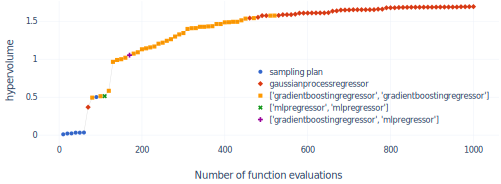
\includegraphics[width=\textwidth]{content/images/wfg1_models}
            \caption{WFG1: Sampling plan bis 60 examples}
            \label{fig:wfg1_models_60}
        \end{subfigure} 

        \caption[The optimization process with dinamic sampling plan and surrogate portfolio.]{The optimization process with dinamic sampling plan and surrogate portfolio. Plots are shown in which step sampling plan was used or which model gives the best accuracy on the test set. More hypervolume is better.}
        \label{fig:changing_models}    
    \end{figure}


    Figure \ref{fig:changing_models} illustrates how improves the solutions for ZDT6 problem. Initially, it could be notest that TutorM considerably outperforms NSGA2 and Hypermapper right from the start of their optimisation process (Fig \ref{fig:zdt6_dist}). TutorM after 300 evaluations, corresponds to the stable near-optimal solution. Besides to interpreter results more involved, non-dominated size should be analysed. ZDT6 landscape has flat regions with local Pareto-front. Hypermapper gets stuck in some of them as evidenced by the serrated graph (Fig \ref{fig:zdt6_ndf}). The drop occurs when discovering a new point in the other Pareto-optimal front. NSGA2 stagnate and comparable to random search due to the many-to-one fitness mapping. Solutions from the population do not have enough sparsity in objective space to detect optimal search direction. TutorM detects global Pareto front straightway and increases Pareto-optimal solutions slowly that alike to solutions from nsga2 with 10k evaluations (Fig \ref{fig:zdt6_front}).

    % === ZDT6
    \begin{figure}
        \centering
        \begin{subfigure}{\textwidth}
            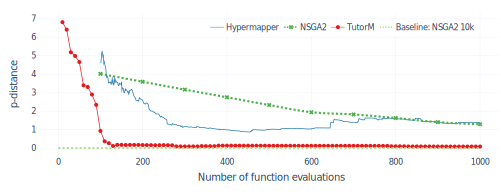
\includegraphics[width=\textwidth]{content/images/zdt6_dist}
            \caption{ZDT6: p-distance to real Pareto-front}
            \label{fig:zdt6_dist}
        \end{subfigure} 
        % \hfill
        
        \begin{subfigure}{\textwidth}
            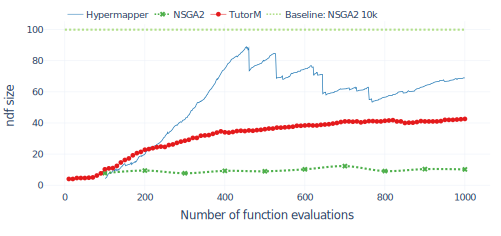
\includegraphics[width=\textwidth]{content/images/zdt6_ndf}
            \caption{ZDT6: Size of a non-dominated subset of an evaluated examples}
            \label{fig:zdt6_ndf}
        \end{subfigure} 

        \begin{subfigure}{\textwidth}
            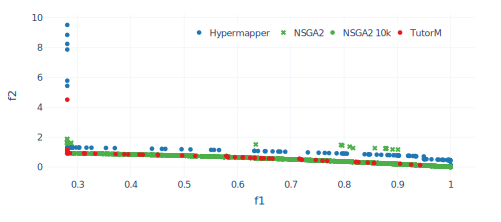
\includegraphics[width=\textwidth]{content/images/zdt6_front}
            \caption{ZDT6: Pareto-front approximation after 1000 function evaluations}
            \label{fig:zdt6_front}
        \end{subfigure} 

        \caption[Comparison of solutions on ZDT6 problem]{A complex comparison of solutions on ZDT6 problem. Final non-dominated points are used to estimate Pareto-optimal solutions.}
        \label{fig:changing_models}    
    \end{figure}


    As shown in Figure \ref{fig:wfg_14}, TutorM could also outperform the MOEA baseline in 10k evaluations(\ref{sub@fig:wfg1_front}). WFG1 has flat landscape regions hence the convergence of genetic algorithms significantly deteriorates. Hypermapper increase count of non-dominated points, regardless it is local optimum and most samples stack in a small region. Nsga2 after 1000 function evaluations also have high-density regions which could be improved with spending more effort to evaluations. The TutorM has several dozen of Pareto-optimal points from all over the budget, that significantly outperforms Hypermapper and nsga2 even with 10k evaluations. 
    From WFG4 use case, all over all approaches gain near-optimal results(\ref{fig:wfg4_front}), but significant advantage over TutorM as it provides an extensive set of points(\ref{fig:wfg4_ndf}) that are well distributed at the Pareto front.


    % === WFG1 and WFG4
    \begin{figure}
        \centering
        \begin{subfigure}{\textwidth}
            \begin{subfigure}{0.5\textwidth}
                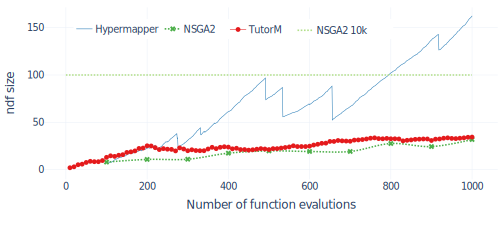
\includegraphics[width=\textwidth]{content/images/wfg1_ndf}
                \caption{WFG1: Size of a non-dominated subset of an evaluated examples}
                \label{fig:wfg1_ndf}
            \end{subfigure} 
            \begin{subfigure}{0.5\textwidth}
                \includegraphics[width=\textwidth]{content/images/wfg1_front}
                \caption{WFG1: Pareto-front approximation}
                \label{fig:wfg1_front}
            \end{subfigure} 
        \end{subfigure} 

        
        % ?\hfill


        \begin{subfigure}{\textwidth}
            \begin{subfigure}{0.5\textwidth}
                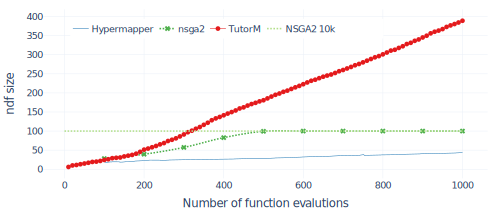
\includegraphics[width=\textwidth]{content/images/wfg4_ndf}
                \caption{WFG4: Size of a non-dominated subset of an evaluated examples}
                \label{fig:wfg4_ndf}
            \end{subfigure} 
            \begin{subfigure}{0.5\textwidth}
                \includegraphics[width=\textwidth]{content/images/wfg4_front}
                \caption{WFG4: Pareto-front approximation}
                \label{fig:wfg4_front}
            \end{subfigure}
        \end{subfigure} 
        
 

        \caption[Comparison of solutions on ZDT6 problem]{A complex comparison of solutions on ZDT6 problem. Final non-dominated points are used to estimate Pareto-optimal solutions.}
        \label{fig:wfg_14}    
    \end{figure}





    \begin{table}[]
        \centering
        \resizebox{\textwidth}{!}{%
        \begin{tabular}{@{}ccccccc@{}}
        \toprule
                                             & \textbf{Metric}        & \textbf{ZDT4} & \textbf{ZDT6} & \textbf{DTLZ4} & \textbf{WFG1} & \textbf{WFG4} \\ \midrule
        \multirow{4}{*}{\textbf{TutorM}}     & \textbf{hypervolume}   & 99,45\%       & 99,01\%       & 99,27\%        & 115,60\%      & 95,95\%       \\
                                             & \textbf{p-distance}    & 1,336         & 0,522         & 0,022          & -             & -             \\
                                             & \textbf{ndf-size}      & 183,022       & 31,528        & 119,308        & 24,158        & 183,244       \\
                                             & \textbf{space-metrics} & 0,103         & 0,142         & 0,186          & 0,129         & 0,032         \\ \midrule
        \multirow{4}{*}{\textbf{NSGA2}}      & \textbf{hypervolume}   & 97,57\%       & 87,46\%       & 95,87\%        & 45,01\%       & 91,87\%       \\
                                             & \textbf{p-distance}    & 1,391         & 1,872         & 0,022          & -             & -             \\
                                             & \textbf{ndf-size}      & 44,000        & 11,455        & 39,900         & 20,164        & 82,436        \\
                                             & \textbf{space-metrics} & 0,176         & 0,355         & 0,268          & 0,228         & 0,038         \\ \midrule
        \multirow{4}{*}{\textbf{Hypermaper}} & \textbf{hypervolume}   & 96,82\%       & 66,95\%       & 81,29\%        & 40,66\%       & 74,09\%       \\
                                             & \textbf{p-distance}    & 2,024         & 1,850         & 0,076          & -             & -             \\
                                             & \textbf{ndf-size}      & 28,908        & 52,746        & 10,743         & 81,512        & 30,158        \\
                                             & \textbf{space-metrics} & 0,1386        & 0,11621       & 0,5282         & 0,0870        & 0,1032        \\ \midrule
        \multirow{4}{*}{\textbf{\begin{tabular}[c]{@{}c@{}}NSGA2\\ 10k eval\end{tabular}}} & \textbf{hypervolume}      & 100,00\% & 100,00\% & 100,00\% & 100,00\% & 100,00\% \\
                                             & \textbf{p-distance}    & 0,152         & 0,256         & 0,002          & -             & -             \\
                                             & \textbf{ndf-size}      & 93,901        & 79,776        & 93,990         & 85,196        & 98,087        \\
                                             & \textbf{space-metrics} & 0,033         & 0,074         & 0,039          & 0,051         & 0,016         \\ \bottomrule
        \end{tabular}%
        }
        \end{table}


% --------------------------------------------------------------------------------------------
% ---------------------       Benchmark 2: Dynamic sampling plan and parameter selection
% --------------------------------------------------------------------------------------------
\section{Benchmark 2: Inner parameters}

    \subsection{Model-tutor parameters}
    \begin{itemize}
        \item \texttt{PredictTutor} class
            \begin{itemize}
                \item Surrogate portfolio
                \item Cross-Validation rounds
                \item Cross-Validation threshold
                \item Train/test split
                \item Test threshold
            \end{itemize}
        \item Optimization search algorithm
        \item Pareto front infill-criteria (Non-dominated score/Solutions combination)
        \item Prediction count
    \end{itemize}

    %! [ Hypermapper baseline; ModelTutor and change quality (grid plot)] iterations

    %! [ Hypermapper baseline; ModelTutor and change quality (bubble chart) ] Deviations



% --------------------------------------------------------------------------------------------
% ---------------------       Benchmark 3: Many-objective optimization, scaling
% --------------------------------------------------------------------------------------------
\section{Benchmark 3: Many-objective optimization. Scaling. RQ1.1}
    For evaluation scalability property for the compositional model, problem XXX was selected.

    Objectives: 1) detect iterative improvement, a convergence of the primary metric 2) time for evaluation

    Usecases: GausianModel, GausianModel + Gradient, GausianModel + random forest, 

    Scale: objectives - 2,4,8,10; params - 2,4,8,10

    % ! [ Hypermapper baseline; X - objectives Y - p-distance/time]



% --------------------------------------------------------------------------------------------
% ---------------------       Benchmark 4: real world scenario
% --------------------------------------------------------------------------------------------
\section{Benchmark 4: Parameter tuning of SVM}

    % ! [ Hypermapper baseline; SVM score in iterations]


% --------------------------------------------------------------------------------------------
% ------------------------------------------------     Discussion 
% --------------------------------------------------------------------------------------------
\section{Discussion}

Up to now, most papers used the
The quality of the results obtained with X was similar to the results obtained with Y, but with significantly fewer exactly evaluated solutions during the optimization process. 


consume an inordinate amount of time.

% \paragraph{Neuroevolution of augmenting topologies}
%  *Training Neural Networks (especially deep ones) is hard and has many issues (non-convex cost functions - local minima, vanishing and exploding gradients etc.).

%  Training Neural Networks (NNs) with Genetic Algorithms (GAs) is not only feasible, there are some niche areas where the performance is good enough to be used frequently. A good example of this is Neuroevolution of augmenting topologies or NEAT, which a successful approach to generating controllers in simple environments, such as games.

%  In the more general case though, the approach does not scale well to large, deep networks with many parameters to tune.

%  Genetic algorithms and other global searches for optimal parameters are robust in ways that gradient-based algorithms are not. For instance, you could train a NN with step function activations, or any other non-differentiable activation functions. They have weaknesses elsewhere. One thing relevant in the case of GAs used for NNs, is that weight parameters are interchangeable in some combinations but heavily co-dependent in other combinations. Merging two equally good neural networks with different parameters - which you would do in cross-over in a GA - will usually result in a third network with poor performance. NEAT's success is partially in finding a way to address that issue by "growing" the NN's connections and matching them up between similar neural networks.

%  Gradient-based approaches are much more efficient. In general, and not just in domain of NNs, if you can calculate gradient of a function with respect to parameters, then you can find optimal parameters faster than most other optimising techniques. An accurate gradient guarantees at least a small improvement from a single evaluation, and most other optimisers fall into a generate-and-retry paradigm which cannot make that kind of guarantee. The weakness of tending to find local optima has turned out not be a major hindrance for the loss functions in NNs, and has been tackled with some degree of success using extensions to basic gradient descent such as momentum, RPROP, Adam etc.

%  In practice on a large multi-layer network, gradient methods are likely orders of magnitude faster than GA searches such as NEAT for finding network parameters. You won't find any GA-trained CNNs that solve ImageNet, or even MNIST, where the GA has found the network weights unaided. However, GAs, or at least some variants of them, are not 100'\%' ruled out. For instance this 2017 blog reviews recent papers including Large-Scale Evolution of Image Classifiers which explores using GAs to discover NN hyperparameters which is an important task in machine learning, and not very tractable using gradient-based methods.
% Test problems  
% Experimental setup
% Results
% Discussion



% non-separable
% or have a deceptive fitness landscape



% On the left side the learning curve of a naive Bayes classifier is shown for the digits dataset. Note that the training score and the cross-validation score are both not very good at the end. However, the shape of the curve can be found in more complex datasets very often: the training score is very high at the beginning and decreases and the cross-validation score is very low at the beginning and increases. On the right side we see the learning curve of an SVM with RBF kernel. We can see clearly that the training score is still around the maximum and the validation score could be increased with more training samples.
% https://scikit-learn.org/0.15/auto_examples/plot_learning_curve.html
    \chapter{Conclusion and Future Work}
    \section{General Conclusion}
    \section{Future Work}
        - BRISE
    
    \bibliographystyle{alpha}
    \bibliography{content/bibliography.bib}

    % must be invoked for correct page numbering in the appendix and all lists
    \backmatter
    

    \appendix
    
    \chapter{Appendix}
        \section{Additional Information}
            % ======= SUMMARY DTLZ
            % Please add the following required packages to your document preamble:
% \usepackage{booktabs}
% \usepackage{multirow}
% \usepackage{graphicx}
\begin{table}[]
    \centering
    \label{tab:dtlz_summary}
    \resizebox{\textwidth}{!}{%
    \begin{tabular}{@{}llllll@{}}
    \toprule
    \textbf{Problem}                & \textbf{Approach}        & $\downarrow$ \textbf{p-distance} & $\uparrow$ \textbf{Hypervolume} \%  & $\uparrow$ \textbf{ndf size} \% & $\uparrow$  \textbf{ndf space} \\ \midrule
    \multirow{4}{*}{DTLZ1} & Baseline       & 0,800           & 100             & 0,24           & 1     \\ \cmidrule(l){2-6} 
    & NSGA2 1k        & \textbf{3,277}  & 56,577          & \textbf{1,56}  & 0,046 \\ \cmidrule(l){2-6} 
    & TutorM          & 51,611          & \textbf{98,163} & 0,54           & 0,058 \\ \cmidrule(l){2-6} 
    & Hypermapper 2.0 & 74,251          & 86,173          & 0,78           & 0,049 \\ \midrule
\multirow{4}{*}{DTLZ2} & Baseline       & 5,19e-06        & 98,603          & 0,24           & 0,39 \\ \cmidrule(l){2-6} 
    & TutorM          & \textbf{0,0004} & \textbf{100}    & \textbf{82,56} & 1     \\ \cmidrule(l){2-6} 
    & NSGA2 1k        & 0,003           & 80,415          & 10          & 0,301 \\ \cmidrule(l){2-6} 
    & Hypermapper 2.0 & 0,058           & 76,103          & 2,84           & 0,063 \\ \midrule
\multirow{4}{*}{DTLZ3} & Baseline       & 0,4           & 100             & 0,24           & 1     \\ \cmidrule(l){2-6} 
    & NSGA2 1k        & \textbf{4,430}  & 74,937          & 0,82           & 0,037 \\ \cmidrule(l){2-6} 
    & TutorM          & 38,735          & \textbf{97,743} & 0,40           & 0,045 \\ \cmidrule(l){2-6} 
    & Hypermapper 2.0 & 92,228          & 95,010          & 0,70           & 0,047 \\ \midrule
\multirow{4}{*}{DTLZ4} & Baseline       & 8,81e-06        & 100             & 0,36           & 1     \\ \cmidrule(l){2-6} 
    & TutorM          & \textbf{0,001}  & \textbf{99,829} & \textbf{30,68} & 0,666 \\ \cmidrule(l){2-6} 
    & NSGA2 1k        & 0,002           & 87,807          & 9,60           & 0,323 \\ \cmidrule(l){2-6} 
    & Hypermapper 2.0 & 0,059           & 64,579          & 1,18           & 0,029 \\ \midrule
\multirow{4}{*}{DTLZ5} & Baseline       & 1,62e-05        & 98,631          & 0,24           & 0,486 \\ \cmidrule(l){2-6} 
    & TutorM          & \textbf{0,0004} & \textbf{100}    & \textbf{80,88} & 1     \\ \cmidrule(l){2-6} 
    & NSGA2 1k        & 0,002           & 81,729          & 10          & 0,434 \\ \cmidrule(l){2-6} 
    & Hypermapper 2.0 & 0,058           & 78,463          & 3,02           & 0,06 \\ \midrule
\multirow{4}{*}{DTLZ6} & Baseline       & 0,009           & 100             & 0,24           & 1     \\ \cmidrule(l){2-6} 
    & TutorM          & \textbf{0,123}  & \textbf{98,064} & 3,70           & 0,142 \\ \cmidrule(l){2-6} 
    & NSGA2 1k        & 1,011           & 54,258          & 2,88           & 0,128 \\ \cmidrule(l){2-6} 
    & Hypermapper 2.0 & 1,657           & 18,355          & 2,22           & 0,084 \\ \midrule
\multirow{4}{*}{DTLZ7} & Baseline       & 2,42e-07        & 99,938          & 0,24           & 0,364 \\ \cmidrule(l){2-6} 
    & TutorM          & \textbf{0,0003} & \textbf{100}    & \textbf{87} & 1     \\ \cmidrule(l){2-6} 
    & NSGA2 1k        & 0,160           & 92,891          & 3,04           & 0,128 \\
    & Hypermapper 2.0 & 0,781           & 91,129          & 2,24           & 0,081 \\ \cmidrule(l){2-6} 
\end{tabular}%
    }
    \caption{Results of 5 repetitions for DTLZ problem set: Function evaluation budget is 1000. The baseline is the NSGA2 with 50000 evaluations (100 population size in 500 generations)}
    \end{table}


            % ======= SUMMARY ZDT
            % Please add the following required packages to your document preamble:
% \usepackage{booktabs}
% \usepackage{multirow}
% \usepackage{graphicx}
\begin{table}[h]
    \centering
    \resizebox{\textwidth}{!}{%
    \begin{tabular}{@{}llllll@{}}
    \toprule
    \textbf{Problem}                & \textbf{Approach}        & $\downarrow$ \textbf{p-distance} & $\uparrow$ \textbf{Hypervolume} \%  & $\uparrow$ \textbf{ndf size} \% & $\uparrow$  \textbf{ndf space} \\ \midrule
    \multirow{4}{*}{ZDT1} & Baseline       & 1,08e-05          & 99,78          & 0,16           & 0,22          \\ \cmidrule(l){2-6} 
                          & TutorM          & \textbf{4,74e-05} & \textbf{100}   & \textbf{90,33} & \textbf{1}    \\ \cmidrule(l){2-6} 
                          & NSGA2 1k        & 0,02              & 89,86          & 9,66           & 0,08          \\ \cmidrule(l){2-6} 
                          & Hypermapper 2.0 & 0,12              & 98,93          & 10,36          & 0,04          \\ \midrule
    \multirow{4}{*}{ZDT2} & Baseline       & 1,04e-14          & 99,79          & 0,16           & 0,29          \\ \cmidrule(l){2-6} 
                          & TutorM          & \textbf{0,00013}  & \textbf{100}   & \textbf{86,87} & \textbf{1}    \\ \cmidrule(l){2-6} 
                          & NSGA2 1k        & 0,01              & 88,78          & 8,82           & 0,06          \\ \cmidrule(l){2-6} 
                          & Hypermapper 2.0 & 0,18              & 97,31          & 5,12           & 0,04          \\ \midrule
    \multirow{4}{*}{ZDT3} & Baseline       & 1,69e-08          & 100            & 0,16           & 0,39          \\ \cmidrule(l){2-6} 
                          & TutorM          & \textbf{0,00012}  & \textbf{99,47} & \textbf{86}    & \textbf{1}    \\ \cmidrule(l){2-6} 
                          & NSGA2 1k        & 0,02              & 89,92          & 9,82           & 0,28          \\ \cmidrule(l){2-6} 
                          & Hypermapper 2.0 & 0,31              & 92,03          & 5,64           & 0,12          \\ \midrule
    \multirow{4}{*}{ZDT4} & Baseline       & 2,04e-05          & 100            & 0,72           & 1             \\ \cmidrule(l){2-6} 
                          & TutorM          & \textbf{0,01}     & \textbf{99,80} & \textbf{50,0}  & \textbf{0,78} \\ \cmidrule(l){2-6} 
                          & NSGA2 1k        & 0,04              & 83,43          & 8,77           & 0,19          \\ \cmidrule(l){2-6} 
                          & Hypermapper 2.0 & 0,90              & 97,32          & 5,42           & 0,11          \\ \midrule
    \multirow{4}{*}{ZDT6} & Baseline       & 0,0003            & 100            & 0,72           & 1             \\ \cmidrule(l){2-6} 
                          & TutorM          & \textbf{0,09}     & \textbf{99,43} & 4,26           & 0,17          \\ \cmidrule(l){2-6} 
                          & Hypermapper 2.0 & 1,12              & 82,86          & \textbf{6,25}  & 0,08          \\ \cmidrule(l){2-6} 
                          & NSGA2 1k        & 1,29              & 83,84          & 1,01           & 0,04          \\ \bottomrule
    \end{tabular}%
    }
    \caption{Results of 5 repetitions for ZDT problem set: Function evaluation budget is 1000. The baseline is the NSGA2 with 50000 evaluations (100 population size in 500 generations)}
    \label{tab:zdt_summary}
    \end{table}

            % ======= SUMMARY WFG
            % Please add the following required packages to your document preamble:
% \usepackage{booktabs}
% \usepackage{multirow}
% \usepackage{graphicx}
\begin{table}[]
    \centering
    \resizebox{!}{11cm}{%
    \begin{tabular}{@{}lllll@{}}
    \toprule
    \textbf{Problem}                & \textbf{Approach}        & $\uparrow$ \textbf{Hypervolume} \%  & $\uparrow$ \textbf{ndf size} \% & $\uparrow$  \textbf{ndf space} \\ \midrule
    \multirow{4}{*}{WFG1} & Baseline       & 100            & 0,72           & 1             \\ \cmidrule(l){2-5} 
                          & TutorM          & \textbf{95,75} & 3,44           & \textbf{0,51} \\ \cmidrule(l){2-5} 
                          & Hypermapper 2.0 & 44,12          & \textbf{10,24} & 0,31          \\ \cmidrule(l){2-5} 
                          & NSGA2 1k        & 30,52          & 3,18           & 0,28          \\ \midrule
    \multirow{4}{*}{WFG2} & Baseline       & 100            & 0,08           & 0,63          \\ \cmidrule(l){2-5} 
                          & TutorM          & \textbf{98,64} & \textbf{29,22} & \textbf{1}    \\ \cmidrule(l){2-5} 
                          & NSGA2 1k        & 85,96          & 6,44           & 0,35          \\ \cmidrule(l){2-5} 
                          & Hypermapper 2.0 & 62,35          & 1,20           & 0,10          \\ \midrule
    \multirow{4}{*}{WFG3} & TutorM          & \textbf{100}   & \textbf{55,50} & \textbf{1}    \\ \cmidrule(l){2-5} 
                          & Baseline       & 99,05          & 0,08           & 0,29          \\ \cmidrule(l){2-5} 
                          & NSGA2 1k        & 84,46          & 9,72           & 0,15          \\ \cmidrule(l){2-5} 
                          & Hypermapper 2.0 & 73,31          & 2,44           & 0,02          \\ \midrule
    \multirow{4}{*}{WFG4} & Baseline       & 100            & 0,72           & 0,60          \\ \cmidrule(l){2-5} 
                          & TutorM          & \textbf{99,28} & \textbf{38,90} & \textbf{1}    \\ \cmidrule(l){2-5} 
                          & Hypermapper 2.0 & 84,39          & 3,26           & 0,06          \\ \cmidrule(l){2-5} 
                          & NSGA2 1k        & 83,95          & 10             & 0,58          \\ \midrule
    \multirow{4}{*}{WFG5} & Baseline       & 100            & 0,20           & 0,24          \\ \cmidrule(l){2-5} 
                          & TutorM          & \textbf{98,01} & \textbf{87,60} & \textbf{1}    \\ \cmidrule(l){2-5} 
                          & Hypermapper 2.0 & 84,83          & 34,74          & 0,06          \\ \cmidrule(l){2-5} 
                          & NSGA2 1k        & 82,70          & 10,00          & 0,18          \\ \midrule
    \multirow{4}{*}{WFG6} & TutorM          & \textbf{100}   & \textbf{52,68} & \textbf{1}    \\ \cmidrule(l){2-5} 
                          & Baseline       & 99,30          & 0,20           & 0,33          \\ \cmidrule(l){2-5} 
                          & NSGA2 1k        & 86,59          & 10             & 0,27          \\ \cmidrule(l){2-5} 
                          & Hypermapper 2.0 & 83,21          & 2,36           & 0,03          \\ \midrule
    \multirow{4}{*}{WFG7} & TutorM          & \textbf{100}   & \textbf{46,30} & \textbf{1}    \\ \cmidrule(l){2-5} 
                          & Baseline       & 99,30          & 0,20           & 0,33          \\ \cmidrule(l){2-5} 
                          & NSGA2 1k        & 86,39          & 10             & 0,26          \\ \cmidrule(l){2-5} 
                          & Hypermapper 2.0 & 83,14          & 2,36           & 0,04          \\ \midrule
    \multirow{4}{*}{WFG8} & Baseline       & 100            & 0,20           & 1             \\ \cmidrule(l){2-5} 
                          & TutorM          & \textbf{95,24} & \textbf{20,70} & \textbf{0,26} \\ \cmidrule(l){2-5} 
                          & Hypermapper 2.0 & 86,74          & 2,80           & 0,07          \\ \cmidrule(l){2-5} 
                          & NSGA2 1k        & 79,63          & 9,54           & 0,20          \\ \midrule
    \multirow{4}{*}{WFG9} & Baseline       & 100            & 0,20           & 0,85          \\ \cmidrule(l){2-5} 
                          & TutorM          & \textbf{92,17} & \textbf{12,92} & \textbf{0,63} \\ \cmidrule(l){2-5} 
                          & Hypermapper 2.0 & 80,80          & 7,30           & 0,24          \\ \cmidrule(l){2-5} 
                          & NSGA2 1k        & 73,56          & 10             & 1             \\ \bottomrule
    \end{tabular}%
    }
    \caption{Results of 5 repetitions for WFG problem set: Function evaluation budget is 1000.
    The baseline is the NSGA2 with 50000 evaluations (100 population size in 500 generations)}
    \label{tab:wfg_summary}
    \end{table}
    
    \printglossary[title=Special Terms, toctitle=List of terms]
    \printglossary[type=\acronymtype,style=long]
    \printglossaries


\end{document}